\documentclass[journal]{IEEEtran}

% Core packages
\usepackage{cite}
\usepackage{amsmath,amssymb}
\usepackage{graphicx}
\usepackage{booktabs}
\usepackage{multirow}
\usepackage{float}
\usepackage{placeins}
\usepackage{flafter}    % a float never appears before its first reference
\usepackage{dblfloatfix}
\usepackage{xcolor}
\usepackage{url}
\usepackage[hidelinks]{hyperref}
\usepackage[T1]{fontenc}
\usepackage[utf8]{inputenc}

\graphicspath{{./images/}}

% Float placement tuning for IEEE two-column layout
\renewcommand{\dbltopfraction}{0.95}
\renewcommand{\topfraction}{0.95}
\renewcommand{\textfraction}{0.05}
\renewcommand{\floatpagefraction}{0.80}
\renewcommand{\dblfloatpagefraction}{0.80}
\setcounter{topnumber}{5}
\setcounter{dbltopnumber}{5}
\setcounter{totalnumber}{8}


\begin{document}
\title{ADMET-Bench: Task-Dependent Performance of GNNs and Pretrained Models in ADMET Prediction}

\author{
\IEEEauthorblockN{
Martin Stamenov\IEEEauthorrefmark{1},
Mila Gjurovska\IEEEauthorrefmark{1},
Viktorija Vodilovska\IEEEauthorrefmark{2} and
Ilinka Ivanoska\IEEEauthorrefmark{1}
}

\IEEEauthorblockA{\IEEEauthorrefmark{1} %1st affiliation
Faculty of Computer Science and Engineering, Ss Cyril and Methodius University, Skopje, N. Macedonia}

\IEEEauthorblockA{\IEEEauthorrefmark{2} %2nd affiliation
Graduate School of Life Sciences, Utrecht University, Utrecht, The Netherlands}

martin.stamenov@students.finki.ukim.mk, mila.gjurovska@students.finki.ukim.mk, v.vodilovska@students.uu.nl, ilinka.ivanoska@finki.ukim.mk

\thanks{Ilinka Ivanoska is the corresponding author.}
\thanks{Martin Stamenov and Mila Gjurovska contributed equally.}
\thanks{Supported by Faculty of Computer Science and Engineering, Skopje, N. Macedonia.}
}

\maketitle

\begin{abstract}
The reliability of structure-based prediction of absorption, distribution, metabolism, excretion, and toxicity (ADMET) properties varies substantially across endpoints, yet many studies compare molecular models without matched tuning or leakage controls. This work benchmarks graph neural networks (GNNs), frozen pretrained molecular representations (ChemBERTa, MolCLR), and fingerprint baselines across six Therapeutics Data Commons endpoints---four pharmacokinetic regression tasks and two toxicity classification tasks---under scaffold-split evaluation. To make the comparison fair, every model family receives a matched 50-trial, validation-selected tuning budget and is evaluated as the median over ten seeds; architecture, hyperparameter, and decision-threshold selection use validation data only, and the held-out test split is used exclusively for final performance estimation, never for any selection. Under this leakage-controlled, budget-matched protocol, \emph{no model family dominates}: differences between families fall within the seed-to-seed range on most endpoints. The GNN is clearly best only on Caco-2 permeability (R$^2 \approx 0.48$), and a controlled ablation shows this advantage comes entirely from auxiliary physicochemical descriptors rather than the graph representation; simple Morgan fingerprints are competitive on hERG (AUC $\approx 0.77$) and give the best median on both clearance endpoints, and MolCLR is best on Tox21. For hepatocyte clearance and half-life, all models yield near-zero or negative R$^2$. Across the six datasets, no hyperparameter-optimization metaheuristic consistently outperforms random search at a 50-trial budget. We further show that common shortcuts---selecting the optimizer on the test set, and reporting single best-trial runs---can substantially inflate a favored model's apparent advantage. ADMET model selection is therefore endpoint-specific, and fair, leakage-controlled, seed-averaged evaluation is essential for realistic assessment of molecular machine-learning models.
\end{abstract}

\begin{IEEEkeywords}
graph neural networks, ADMET prediction, molecular property prediction, scaffold-split, pretrained models, drug discovery, benchmarking
\end{IEEEkeywords}


\section{Introduction}
\label{sec:intro}

\IEEEPARstart{P}{redicting} molecular ADMET (Absorption, Distribution, Metabolism, Excretion, and Toxicity) properties is a central task in computational drug discovery, enabling early identification of promising candidates and flagging safety liabilities before costly synthesis and \emph{in vivo} testing~\cite{zhang2025admet}. Graph Neural Networks (GNNs) have become prominent in this domain by treating molecules as graphs in which atoms serve as nodes and bonds as edges, enabling task-specific learning through message passing that encodes both local chemical motifs and global topological patterns inaccessible to fixed-length descriptors~\cite{gilmer2017neural, yang2019dmpnn, attentiveFP}.

\begin{table*}[!t]
\centering
\caption{Summary of representative molecular property prediction methods. Performance is reported for selected TDC ADMET tasks under scaffold-split where available. GNN = Graph Neural Network, FP = Fingerprint, TF = Transformer, PT = Pretrained.}
\label{tab:related_work_summary}
\scriptsize
\begin{tabular}{llp{5.5cm}l}
\toprule
\textbf{Method} & \textbf{Type} & \textbf{Key Approach} & \textbf{Ref.} \\
\midrule

\multicolumn{4}{l}{\emph{Fingerprint-Based Methods}} \\
\midrule
MapLight & FP+ML & Morgan FP with RF and SVM on node embeddings & \cite{maplight} \\
FCA & Ensemble & Weighted combination of RF, XGBoost, and SVM & \cite{cfa} \\
RDKit2D + MLP & FP+ML & 200 physicochemical descriptors with MLP & \cite{rdkit2d_mlp} \\

\midrule
\multicolumn{4}{l}{\emph{Graph Neural Networks}} \\
\midrule
AttentiveFP & GNN & GCN/GAT layers with GRU-based attention readout & \cite{attentiveFP} \\
GCN & GNN & Multi-layer graph convolution with mean pooling & \cite{kipf2017gcn} \\
GIN & GNN & Graph isomorphism layers for WL-test expressivity & \cite{xu2019gin} \\
D-MPNN & GNN & Directed message passing on bonds & \cite{yang2019dmpnn} \\
MPNN++ & GNN & Enhanced message passing ($\sim$10M params) & \cite{miniMol} \\

\midrule
\multicolumn{4}{l}{\emph{Pretrained GNN Models}} \\
\midrule
Attr.\ Masking & GNN+SSL & Node/edge attribute masking for pretraining & \cite{attrMasking} \\
GraphCL & GNN+SSL & Graph-level contrastive learning with augmentations & \cite{contrativeLearning} \\
MolCLR & GNN+SSL & Molecular contrastive learning of representations & \cite{molclr} \\
MolE & GNN+FM & Multi-task pretrained GNN encoder & \cite{molE} \\
DeepMol & GNN+FM & Deep molecular representation learning & \cite{deepMol} \\
MiniMol & GNN+FM & Compact pretrained molecular model using MPNN++ & \cite{miniMol} \\

\midrule
\multicolumn{4}{l}{\emph{Pretrained Transformer Models}} \\
\midrule
ChemBERTa-2 & TF & RoBERTa pretrained on 77M SMILES (ZINC) & \cite{chemberta2} \\
MolBERT & TF & BERT with SMILES and physicochemical objectives & \cite{molbert} \\

\bottomrule
\end{tabular}
\end{table*}

Beyond GNNs, a diverse range of AI and machine learning approaches has been applied to ADMET prediction. Pretrained molecular encoders such as ChemBERTa~\cite{chemberta2} and MolCLR~\cite{molclr} leverage self-supervised learning on large molecular corpora to produce reusable molecular representations for downstream tasks. Classical fingerprint-based methods, including Morgan (ECFP) fingerprints~\cite{rogers2010ecfp} paired with traditional ML or MLP predictors, remain competitive baselines on many benchmarks~\cite{maplight, rdkit2d_mlp}. Although these approaches differ substantially in architecture and encoding strategy, all evaluated model families in this study rely exclusively on molecular structure as input, representing the same underlying 2D molecular graph or SMILES string~\cite{weininger1988smiles} through different feature representations. GNNs operate directly on molecular graphs, fingerprint methods encode local substructures into fixed-length vectors, and transformer-based models learn contextual embeddings from SMILES sequences. Across these paradigms, strong predictive performance has been reported in the literature, often achieving state-of-the-art results on individual tasks~\cite{huang2021therapeuticsdatacommonsmachine}.

Despite this progress, model selection in practice remains unclear. Different models perform inconsistently across tasks and molecular structures, and most published studies optimize performance for individual architectures or compare methods under different splits and experimental conditions, making direct comparison unreliable~\cite{wu2018moleculenet, yang2019dmpnn}. Crucially, many works rely on random data splits, which allow structurally similar molecules to appear in both training and test sets. This leads to overly optimistic performance estimates that do not reflect the real-world scenario of predicting properties for new chemical scaffolds, where distribution shift is inevitable. As a result, practitioners still lack consistent guidance on model selection, endpoint-specific reliability, and the conditions under which molecular structure alone provides sufficient predictive information \cite{wu2018moleculenet, huang2021therapeuticsdatacommonsmachine}.

Evaluation protocols fundamentally influence conclusions about predictive performance in molecular machine learning, particularly in settings where generalization to unseen chemical scaffolds is required. However, the extent to which evaluation protocol alters both model and optimizer rankings remains insufficiently understood. Scaffold-based splitting~\cite{doi:10.1021/jm9602928}, which partitions compounds by core ring structures, serves as a realistic evaluation protocol that reflects prospective drug discovery campaigns where models must generalize to novel chemical series. In this work, we investigate how the predictive performance of molecular AI models depends on the underlying task and evaluation protocol, with a focus on identifying when molecular structure alone provides sufficient signal. This issue is particularly important for pharmacokinetic endpoints such as clearance and half-life, where inaccurate predictions can affect compound prioritization before experimental validation. Models that appear accurate under weak evaluation protocols may therefore provide misleading support for early-stage screening decisions.

For this reason, benchmarking should identify not only which model performs best, but also which endpoints are predictable from molecular structure under realistic scaffold-shift conditions. This motivates endpoint-specific model selection, where the modeling approach is chosen according to the biological and experimental characteristics of the endpoint. From a biomedical informatics perspective, ADMET predictors act as decision-support components in early-stage drug-discovery pipelines that inform AI-supported compound prioritization. If such models are evaluated under overly optimistic protocols, they may produce overconfident predictions for novel chemical scaffolds and misguide prioritization. Understanding endpoint-specific reliability under scaffold shift is therefore essential for trustworthy AI in translational drug-discovery workflows, shifting the focus from maximizing aggregate benchmark scores toward assessing when an ADMET model is reliable enough to support compound-prioritization decisions and when its predictions should be treated as low-confidence evidence.

The main contributions of this study are as follows:

\begin{itemize}
    \item We present a systematic benchmark of graph-based, fingerprint-based, and pretrained molecular representation models across six ADMET endpoints from the TDC benchmark.

    \item We evaluate model performance under scaffold-split conditions, enabling a more realistic assessment of generalization to structurally distinct compounds.

    \item We compare model behavior across endpoints with different biological characteristics, showing how predictive performance varies between permeability, toxicity, cardiotoxicity, clearance, and half-life tasks.

    \item We assess seven hyperparameter-optimization strategies for the GNN across six ADMET endpoints under a common 50-trial budget---an analysis kept separate from the matched-budget model-family comparison---and examine whether optimizer choice consistently improves performance.

    \item We identify endpoint-specific cases where molecular structure provides sufficient predictive signal, as well as cases where structure-only representations remain limited, motivating the use of biological or assay-level information in future ADMET models.
\end{itemize}

The remainder of this paper is organized as follows.
Section~II reviews related work on ADMET prediction, molecular representation learning, scaffold-split evaluation, and hyperparameter optimization for molecular machine learning.
Section~III describes the materials and methods, including the selected TDC datasets, molecular representations, model families, scaffold-split protocol, hyperparameter optimization strategies, and evaluation metrics.
Section~IV presents the experimental results across regression and classification endpoints and analyzes model-family and optimizer performance.
Section~V discusses the implications of endpoint-dependent model behavior, scaffold-split generalization, and the limitations of structure-only molecular representations.
Finally, Section~VI concludes the paper and outlines directions for future work.

\section{Related Work}
\label{sec:related}

\subsection{ADMET Prediction}

The TDC ADMET benchmark~\cite{huang2021therapeuticsdatacommonsmachine} has become the standard evaluation platform for molecular property prediction. Table~\ref{tab:related_work_summary} summarizes representative approaches from the TDC leaderboard and the broader literature.

The TDC leaderboards~\cite{tdc_admet_leaderboard} reveal that several top-performing approaches rely on comparatively simple architectures. MapLight~\cite{maplight} uses random forests and SVMs on node embeddings, while RDKit2D+MLP~\cite{rdkit2d_mlp} passes 200 physicochemical descriptors through a standard multi-layer perceptron. On certain datasets, even Random Forest or XGBoost achieves top results, motivating ensemble approaches such as FCA~\cite{cfa}, which combines multiple classifiers via weighted voting.


\begin{figure*}[!t]
    \centering
    \includegraphics[width=0.70\textwidth,height=0.58\textheight,keepaspectratio]{architecture.png}
    \caption{Modular benchmarking architecture for evaluating molecular graph neural networks and pretrained models on ADME and toxicity prediction tasks. The framework consists of three layers: a benchmark orchestration layer coordinating datasets and experimental configurations, a model execution layer evaluating multiple neural architectures, and an evaluation pipeline.}
    \label{fig:benchmark-framework}
\end{figure*}

Among GNN-based methods, AttentiveFP~\cite{attentiveFP} employs GCN/GAT layers with GRU-based attention readout, achieving top-5 results on many TDC datasets. Standard architectures appearing prominently in molecular benchmarks include GCN~\cite{kipf2017gcn}, GIN~\cite{xu2019gin}, and D-MPNN~\cite{yang2019dmpnn}, which operates on bond-level rather than atom-level messages.

Self-supervised pretraining has been adapted from NLP to molecular graphs via two main paradigms: attribute masking~\cite{attrMasking}, which reconstructs removed node or edge features, and contrastive learning~\cite{contrativeLearning}, which trains encoders to produce similar embeddings for augmented views of the same molecule. MolCLR~\cite{molclr} extends contrastive learning with three graph augmentation strategies (atom masking, bond deletion, subgraph removal), demonstrating improved downstream ADMET prediction compared to training from scratch.

These techniques underpin most pretrained molecular representation models, which follow a common paradigm: self-supervised pretraining on large unlabeled corpora, optional multi-task supervised training, and task-specific fine-tuning. Representative examples include DeepMol~\cite{deepMol} and MolE~\cite{molE}. ChemBERTa~\cite{chemberta2} takes a distinct approach, applying a RoBERTa transformer to SMILES strings pretrained on 77M molecules from ZINC-15~\cite{sterling2015zinc15}, while MolBERT~\cite{molbert} combines SMILES masked language modeling with auxiliary physicochemical objectives. A practical concern with pretrained molecular representation models is their large parameter count; MiniMol~\cite{miniMol} addresses this by using MPNN++ ($\sim$10M parameters) to achieve competitive TDC performance at substantially lower computational cost.

\paragraph{Scaffold Split Challenges}
Transformer-based models frequently show severe generalization drops under scaffold splitting, with strong validation scores that collapse toward chance-level performance on held-out scaffolds~\cite{yang2019dmpnn,chemberta2}. Wu et al.~\cite{wu2018moleculenet} introduced MoleculeNet with scaffold-splitting to more faithfully reflect prospective drug discovery generalization. This observation is revisited in Section~\ref{sec:results}, where the experimental results show that on Tox21 NR-AR the pretrained encoders reach high validation AUC that does not transfer to the scaffold-split test set (ChemBERTa $\approx0.92$ validation~$\to$~$0.714$ test median; MolCLR $\approx0.90$~$\to$~$0.722$).


\subsection{Hyperparameter Optimization for Molecular ML}

HPO is a key performance driver in molecular ML, where small, noisy datasets amplify sensitivity to hyperparameter configuration. Bergstra and Bengio~\cite{bergstra2012random} established Random Search as a strong baseline, showing it outperforms grid search when only a subset of hyperparameters is influential. Bayesian methods such as TPE~\cite{bergstra2011tpe}, implemented in Optuna~\cite{akiba2019optuna}, improve sample efficiency by modeling the hyperparameter-performance relationship, making them attractive under limited trial budgets.

Population-based metaheuristics, including PSO~\cite{kennedy1995pso}, GA~\cite{holland1975ga}, and ABC~\cite{karaboga2005abc}, provide broader exploration, but may require larger budgets to converge. SA~\cite{saopt} offers a middle ground by accepting suboptimal moves early to escape local optima. Despite their widespread use in combinatorial optimization, systematic comparisons of these HPO strategies for molecular property prediction remain scarce, particularly under scaffold-split protocols, motivating our evaluation of multiple optimization approaches within a unified ADMET benchmark.


\subsection{Challenges in Molecular ML: Distribution Shifts and Generalization}
Beyond the scaffold-split sensitivity discussed above, molecular property prediction faces additional generalization challenges that compound evaluation difficulty. First, ADMET datasets are typically small (hundreds to low thousands of compounds), which amplifies variance across data splits and makes HPO-selected configurations sensitive to the specific training fold~\cite{wu2018moleculenet}. Second, the relationship between molecular structure and pharmacokinetic endpoints is often indirect: properties such as clearance and half-life depend on enzyme kinetics, transporter activity, and protein binding factors not explicitly encoded in molecular graphs or SMILES strings~\cite{obach1999prediction}. Third, class imbalance~\cite{he2009imbalanced} in toxicity assays (e.g., 4.2\% positive rate in Tox21 NR-AR) biases standard loss functions toward the majority class, a problem that persists in our experiments where no explicit class reweighting is applied.

These compounding factors mean that reported model rankings can shift substantially depending on dataset size, splitting protocol, and evaluation metric. Robust benchmarking therefore requires multi-seed validation, paired effect-size estimation, and confidence intervals, practices that remain inconsistent in molecular ML. Our framework enforces all three across every comparison.



\section{Materials and Methods}
\label{sec:methods}

\subsection{Framework Overview}
\label{sec:framework}

To compare model families under realistic generalization conditions, we use a benchmarking framework (Fig.~\ref{fig:benchmark-framework}) that applies the same scaffold partitions, datasets, and metrics across the GNN and the frozen-pretrained/fingerprint pipelines. The framework coordinates dataset loading, scaffold-split partitioning, model training, metric computation, and statistical analysis.
The statistical analysis includes repeated runs with different random seeds, aggregation of across-seed summary statistics (medians and ranges), comparison of model families across endpoints, and confidence-interval-based comparison of hyperparameter optimization strategies against a Random Search baseline.
Fixing the splits, datasets, and metrics across models removes split- and metric-related confounds that complicate cross-study comparison in molecular ML~\cite{wu2018moleculenet}, so that observed differences reflect model characteristics rather than experimental artifacts. The design separates experiment orchestration, model execution, and evaluation into independent components, so new algorithms, architectures, or datasets can be added without modifying the evaluation logic.


\subsection{Datasets and Evaluation Protocol}
\label{sec:datasets}

We evaluate all models on six molecular property prediction tasks drawn from the Therapeutics Data Commons (TDC) ADMET benchmark~\cite{huang2021therapeuticsdatacommonsmachine}, covering four pharmacokinetic (ADME) regression tasks and two toxicity classification tasks. This evaluation protocol reflects practical drug discovery scenarios, where models are required to generalize to novel chemical series. Fig.~\ref{fig:class-distribution} provides an overview of data provenance and class composition across all six datasets.

\subsubsection{ADME Regression Tasks}

\paragraph{Caco-2 Permeability (Caco2\_Wang)}
The Caco-2 cell monolayer assay is the gold-standard \emph{in vitro} surrogate for human intestinal absorption~\cite{artursson1991caco2}. High apparent permeability ($P_{app} > 10^{-6}$ cm/s) is associated with good oral bioavailability. The dataset, curated by Wang et al.\ and provided through the Therapeutics Data Commons~\cite{huang2021therapeuticsdatacommonsmachine}, contains \textbf{910 compounds} with target values expressed in log(cm/s) units. Caco-2 showed the strongest regression performance in our benchmark, likely because permeability is closely related to molecular size, lipophilicity, and hydrogen-bonding capacity, which are represented directly in molecular graphs.

\paragraph{Half-Life Prediction (Half\_Life\_Obach)}
Plasma half-life ($t_{1/2}$, hours) determines dosing frequency and is essential for designing drugs with adequate therapeutic windows. However, half-life is a composite pharmacokinetic parameter influenced not only by molecular structure, but also by volume of distribution, protein binding fraction, and individual patient variability~\cite{obach1999prediction}. The dataset is drawn from the Obach FDA-approved drug collection and contains \textbf{667 compounds} spanning a wide dynamic range (0.5-100$+$ hours). We apply a log transformation before standardization to reduce target skewness.

\begin{figure*}[!t]
    \centering
    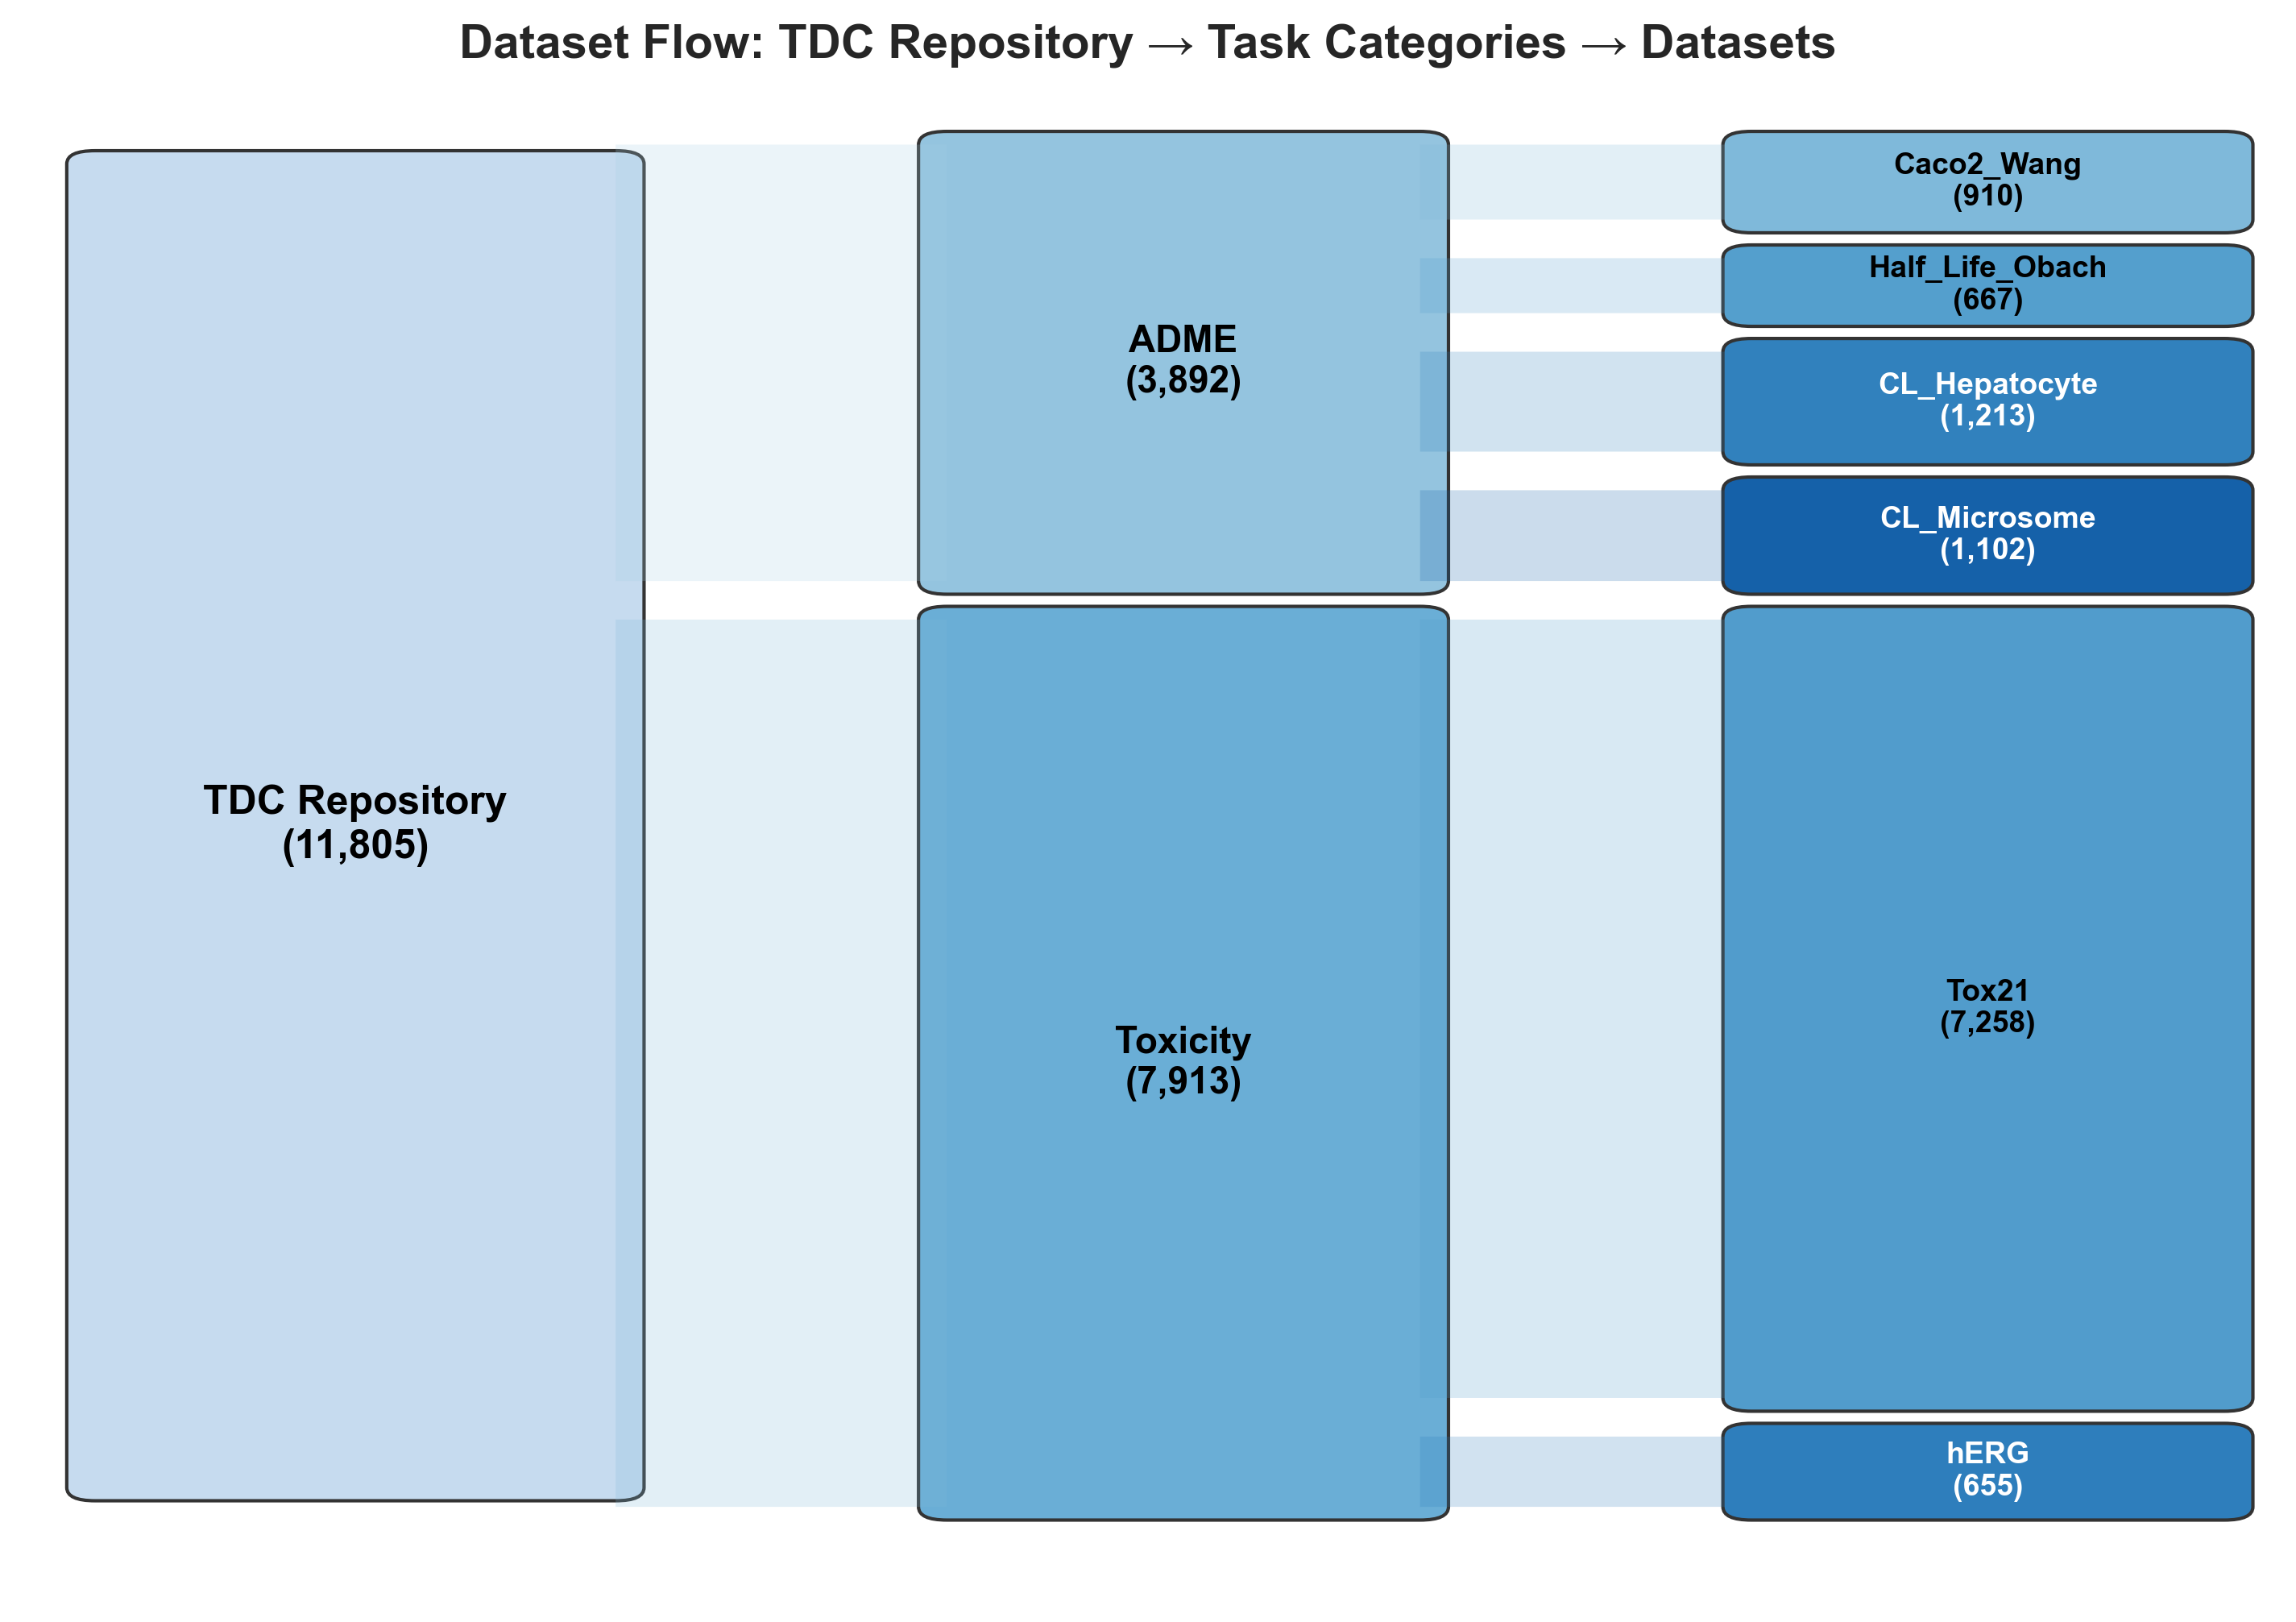
\includegraphics[width=0.9\textwidth,height=0.42\textheight,keepaspectratio]{sankey-diagram.png}
    \caption{Overview of data source and task labels. This flowchart details the $11{,}805$ total instances catalogued in the TDC Repository. After removing molecules with invalid SMILES or failed graph conversion, $10{,}627$ molecules are retained for training and evaluation.}
    \label{fig:class-distribution}
\end{figure*}

\paragraph{Hepatocyte Clearance (Clearance\_Hepatocyte\_AZ)}
Intrinsic clearance measured in freshly isolated human hepatocytes ($\mu$L/min/10$^6$ cells) captures both phase-I and phase-II metabolic routes and is the most physiologically relevant \emph{in vitro} metabolic stability assay~\cite{riley2005unified}. The dataset was generated internally at AstraZeneca and is distributed through TDC~\cite{huang2021therapeuticsdatacommonsmachine}, comprising \textbf{1\,213 proprietary compounds}. This dataset yielded the weakest regression performance in our benchmark, with GNN models producing negative R$^2$ values, suggesting that, within this benchmark, molecular structure alone was insufficient to explain the observed variance in hepatic metabolism (see Section~\ref{sec:results}).

\paragraph{Microsomal Clearance (Clearance\_Microsome\_AZ)}
Human liver microsomal assays ($\mu$L/min/mg protein) measure primarily cytochrome P450-mediated (CYP) oxidative metabolism; they offer higher throughput than hepatocyte assays, but capture only phase-I reactions~\cite{obach2006trend}. The AstraZeneca dataset contains \textbf{1\,102 compounds}. Like hepatocyte clearance, microsomal clearance values are log-transformed and then standardized using train-set statistics.

\subsubsection{Toxicity Classification Tasks}

\paragraph{Tox21 Nuclear Receptor: Androgen Receptor (Tox21 NR-AR)}
The Tox21 initiative~\cite{tox21data} assembled a large multi-assay toxicology panel to enable high-throughput environmental hazard screening. We use the \textbf{NR-AR} assay (androgen receptor agonism), which identifies compounds that can disrupt androgen signaling. The TDC catalogue lists \textbf{7\,258 compounds} (6\,533 after graph conversion), of which only $\approx4.2\%$ are active (positive) samples across the full corpus (see Fig.~\ref{fig:class-distribution}), making this the most class-imbalanced task in our benchmark; the scaffold-split test set has a slightly higher positive rate of $\approx4.9\%$.


\paragraph{hERG Cardiotoxicity (hERG)}
Blockade of the hERG potassium ion channel is the predominant mechanism of drug-induced QT interval prolongation and potentially fatal cardiac arrhythmias, and the hERG assay is a mandatory safety screen in preclinical drug development~\cite{sanguinetti2006herg}. The TDC hERG dataset contains \textbf{655 compounds} with binary blocker/non-blocker labels; approximately 69\% of compounds are blockers (a roughly 69/31 class split), making this a considerably more balanced classification task than Tox21 NR-AR.

\paragraph{Splitting and evaluation protocol}
We use the TDC scaffold-split function, which partitions compounds by Bemis-Murcko scaffolds~\cite{doi:10.1021/jm9602928} so that molecules with structurally distinct core rings appear in different folds. Scaffold-based splitting approximates prospective deployment conditions, where a model must generalize to structurally distinct compound families not seen during training. We further subdivide the scaffold-held training partition into training and validation at the \emph{molecule} level: observations are grouped by canonical SMILES, and each unique molecule---with all of its measurements---is assigned to either training or validation using a fixed random seed (42), so that no molecule can occur in both partitions. A fixed fraction (10\%) of the unique molecules forms the validation set, used for early stopping and model selection; the held-out scaffold test set is left unchanged. The final split proportions are approximately 70/8/22 (train/validation/test) across all datasets.
Because scaffold splitting assigns entire scaffold groups to the same partition, the exact proportions may vary slightly across datasets.

During hyperparameter optimization (HPO), the test split remains \emph{fully held out}; model selection is performed solely on the validation metric. Final performance is reported once on the test split after HPO is complete, preventing any implicit information leakage from repeated test-set evaluations.

\paragraph{Target transformations}
For the three skewed regression tasks (Half-Life, Hepatocyte and Microsomal Clearance) we apply $y' = \log(\max(y, \epsilon))$, where $\epsilon = 10^{-3}$, followed by z-score normalization using training-set statistics. Caco-2 targets are already in log(cm/s) units, so only z-score normalization is applied. All normalization parameters are computed exclusively on the training fold and reused for validation and test sets to prevent data leakage. Classification targets are kept as binary integers (0/1) without transformation.

\subsection{Model Families}
\label{sec:model_families}

This comparison allows us to evaluate whether task-specific learning provides advantages over frozen pretrained molecular representations and fixed fingerprint baselines. We evaluate three distinct model paradigms under the same scaffold splits and evaluation metrics.

\paragraph{GNN models}
We employ graph neural networks trained end-to-end on each task. The GNN backbone is based on stacked GraphConv layers~\cite{morris2019wlgnn} with batch normalization, ReLU activation, and additive residual connections between successive layers, selected through a preliminary architecture comparison across eight GNN variants (Section~\ref{sec:arch_selection}). Each molecule is represented as a molecular graph constructed from SMILES using RDKit. Atom features include atomic number, degree, formal charge, hybridization, aromaticity, ring membership, hydrogen count, and atomic mass (8 features); no bond features are used. The GNN encoder produces node embeddings aggregated into a graph-level representation using concatenated global mean and max pooling. Before the prediction head, this pooled graph representation is concatenated with a small vector of structure-derived physicochemical descriptors computed with RDKit (15 descriptors for the ADME regression and toxicity tasks: molecular weight, cLogP, hydrogen-bond donors and acceptors, topological polar surface area, rotatable bonds, aromatic and aliphatic ring counts, molar refractivity, Bertz complexity, heteroatom count, and four Lipinski-rule flags; a 7-descriptor subset for Caco-2). These descriptors are derived from molecular structure alone and add no biological or assay information; they are provided only to the GNN and not to the pretrained or fingerprint baselines (see Section~\ref{sec:discussion}). The combined representation is passed to an MLP prediction head with batch normalization and optional dropout. To regularize the small Caco-2 dataset, the GNN additionally applies dropout ($0.5$) and Gaussian target-label noise ($\sigma=0.05$) for that endpoint only. GNN models undergo full hyperparameter optimization (Section~\ref{sec:model_training}).

\paragraph{Pretrained models}
We evaluate two pretrained molecular encoders representing the two major pretrained molecular model paradigms shown in Table~\ref{tab:related_work_summary}. We use SMILES-based transformer models such as ChemBERTa~\cite{chemberta2} and graph-based contrastive models such as MolCLR~\cite{molclr} as representative examples of sequence-based and graph-based pretrained approaches, rather than as an exhaustive list of all available pretrained molecular models. For pretrained encoders, we use a frozen encoder and trainable MLP head setting: embeddings are extracted once per molecule, and an MLP head is trained on the train split with early stopping on the validation split. Its hyperparameters (hidden-layer widths, learning rate, and $L_2$ regularization) are selected by a 50-trial validation-based random search, matching the per-endpoint tuning budget given to the GNN so that all model families receive comparable optimization opportunity. This frozen-encoder protocol isolates the quality of the pretrained representation from encoder fine-tuning while giving the downstream head the same tuning budget as the other model families.

\paragraph{Fingerprint baselines}
We evaluate two fingerprint-based approaches: (i) Morgan fingerprints (ECFP)~\cite{rogers2010ecfp} with an MLP predictor, and (ii) MolE-style learned fingerprints (MolE-FP) with an MLP predictor. The MolE-FP baseline is implemented as Morgan fingerprints followed by a learned projection inspired by the MolE approach~\cite{molE}, rather than the original pretrained MolE encoder. These fixed molecular descriptors serve as baselines representing the classical cheminformatics approach to molecular property prediction. All baselines use the same dataset splits, evaluation metrics, and 50-trial validation-based head tuning as the GNN experiments.




\subsection{Model Training and Configuration}
\label{sec:model_training}

\paragraph{GNN Training}
All GNN models were trained using the Adam optimizer with a batch size of 32. During HPO, models were trained for a maximum of 50 epochs per trial with early stopping (patience = 12). Regression models were optimized using mean squared error (MSE) loss, while classification models used binary cross-entropy (BCE) loss with logits. Gradient clipping was applied with a maximum norm of 1.0. Table~\ref{tab:search_space} defines the hyperparameter search space. The three MLP-head widths are constrained to be non-increasing (Layer~1~$\geq$~Layer~2~$\geq$~Layer~3), so a sampled triple is sorted in descending order before use, yielding the funnel-shaped prediction head used throughout.

\begin{table}[!t]
\centering
\caption{Hyperparameter Search Space for GNN Models. The three MLP-head layer widths are sampled independently and then sorted in descending order (Layer~1~$\geq$~Layer~2~$\geq$~Layer~3) to yield a funnel-shaped prediction head.}
\label{tab:search_space}
\small
\begin{tabular}{ll}
\toprule
\textbf{Hyperparameter} & \textbf{Search Space} \\
\midrule
Hidden Dimensions & \{64, 96, 128, 192, 256, 384, 512\} \\
Number of Layers & \{3, 4, 5, 6, 7\} \\
Learning Rate & [1e-4, 1e-2] (log-uniform) \\
Weight Decay & [1e-6, 1e-2] (log-uniform) \\
MLP Head Layer 1 & \{128, 192, 256, 384, 512\} \\
MLP Head Layer 2 & \{64, 96, 128, 192, 256\} \\
MLP Head Layer 3 & \{32, 48, 64, 96, 128\} \\
\bottomrule
\end{tabular}
\end{table}

\paragraph{Optimization algorithms}
We evaluate seven HPO strategies, Random Search~\cite{bergstra2012random}, Particle Swarm Optimization (PSO)~\cite{kennedy1995pso}, Artificial Bee Colony (ABC)~\cite{karaboga2005abc}, Genetic Algorithm (GA)~\cite{holland1975ga}, Simulated Annealing (SA)~\cite{saopt}, Hill Climbing (HC)~\cite{russell2010aima}, and Tree-structured Parzen Estimator (TPE)~\cite{akiba2019optuna}. For population-based methods (PSO, GA, ABC), a population size of 16 is used. SA is initialized with temperature $T_0 = 1.0$ and exponential cooling ($\alpha = 0.99$). TPE uses Optuna's default of 10 startup trials with median pruning. All NiaPy-based~\cite{niapy} methods operate over the 7-dimensional search space in Table~\ref{tab:search_space}. TPE (Optuna) searches a separate space over hidden dimension, number of layers, learning rate, weight decay, and dropout rate $\in [0.0, 0.5]$. Each algorithm is allocated 50 trials per dataset, giving 2{,}100 GNN training runs from the optimizer comparison alone (seven optimizers $\times$ six datasets $\times$ 50 trials); together with the preliminary architecture-selection screen (240 runs: eight architectures $\times$ six endpoints $\times$ five configurations) and the ten-seed validation (60 runs), the study comprises approximately 2{,}400 training runs in total.

\begin{table}[!t]
\centering
\caption{Dataset statistics and evaluation metrics (TDC ADMET). ``TDC'' shows compounds catalogued; ``Used'' shows those retained after filtering. RMSE is the primary per-dataset regression metric; the scale-invariant R$^2$ is additionally used for cross-model comparison in Table~\ref{tab:model_comparison}.}
\label{tab:dataset_stats}
\small
\begin{tabular}{lccccc}
\toprule
\textbf{Dataset} & \textbf{Type} & \textbf{TDC} & \textbf{Used} & \textbf{Split} & \textbf{Metric} \\
\midrule
Caco2\_Wang & Regr. & 910 & 819 & Scaffold & RMSE \\
Half\_Life & Regr. & 667 & 601 & Scaffold & RMSE \\
Clear.\_Hep. & Regr. & 1,213 & 1,092 & Scaffold & RMSE \\
Clear.\_Mic. & Regr. & 1,102 & 992 & Scaffold & RMSE \\
Tox21 (NR-AR) & Class. & 7,258 & 6,533 & Scaffold & AUC \\
hERG & Class. & 655 & 590 & Scaffold & AUC \\
\bottomrule
\end{tabular}
\end{table}

\subsection{Experimental Setup}
\label{sec:experimental_setup}

\paragraph{Datasets}
Table~\ref{tab:dataset_stats} summarizes the dataset characteristics across all six tasks.

\paragraph{Evaluation metrics}
Model performance is assessed using RMSE, R$^2$, and MAE for ADME regression tasks, and AUC-ROC and F1-score for toxicity classification tasks. AUC-ROC is the primary ranking metric for classification; for the severely imbalanced Tox21 (NR-AR) endpoint ($\approx$5\% positives) we additionally treat PR-AUC as a co-primary metric, because ROC-AUC can remain high even when practical detection of the minority class is weak. AUC-ROC is also the classification metric used in the paired optimizer comparison (Table~\ref{tab:best_results}); F1 is reported in addition because it is more sensitive to the minority class under strong class imbalance.

\paragraph{Multi-seed validation}
To quantify robustness, we retrain the best HPO-selected configuration per dataset across ten seeds $[42, 123, 456, 789, 1011, 2022, 3033, 7, 99, 2718]$. We report the median and the full min--max range across seeds; the median is used because the best configuration diverges on a minority of seeds for the weakly-learnable endpoints, which makes the across-seed mean unrepresentative.

\paragraph{HPO algorithm comparison}
We compare each optimizer against the Random Search baseline using paired per-endpoint differences across the six datasets rather than null-hypothesis significance tests. For every endpoint we take the difference in that endpoint's primary test metric (R$^2$ for regression, AUC-ROC for classification), oriented so that positive values favor the optimizer. Because these metrics lie on incomparable scales and the regression R$^2$ is occasionally pathologically negative, a raw mean difference is not a sound summary; we therefore report (i) the win/tie/loss count with an exact two-sided sign test on wins-versus-losses (ties dropped), (ii) a scale-free, direction-normalized paired effect---each endpoint's difference divided by the spread of all seven optimizers on that endpoint, then averaged over the six endpoints---and (iii) two sensitivity variants that recompute the mean paired difference with R$^2$ clipped to $[-1,1]$ and floored at $0$ (AUC untouched). All 95\% confidence intervals are $10{,}000$-resample percentile bootstraps over the six paired differences. The paired unit is the dataset ($n=6$), and all comparisons use final held-out test performance obtained after HPO model selection on the validation split. With only six paired observations, null-hypothesis significance tests are underpowered, so we read these measures descriptively, summarizing the magnitude and the consistency of any improvement over Random Search.

\paragraph{Implementation}
The implementation was carried out in Python~$\geq$~3.8 using PyTorch~$\geq$~2.0, PyTorch Geometric~$\geq$~2.3, RDKit~$\geq$~2022.9, PyTDC~$\geq$~0.4, NiaPy~$\geq$~2.0~\cite{niapy}, Optuna~$\geq$~3.0, and Transformers~$\geq$~4.30.
All experiments were executed on a workstation equipped with an Intel Core i7-8700K CPU running at 3.70~GHz, 16~GB of RAM, and an NVIDIA GeForce RTX 3060 GPU.
The total runtime required to complete all experimental runs was approximately 45~hours.


\section{Results}
\label{sec:results}

\subsection{Task-Level Performance on ADMET Endpoints}
\label{sec:task_level}

Table~\ref{tab:model_comparison} presents the performance of all model families across the six ADMET tasks. Fig.~\ref{fig:foundation_ranking} provides a visual summary of relative model rankings.

\begin{figure}[!t]
    \centering
    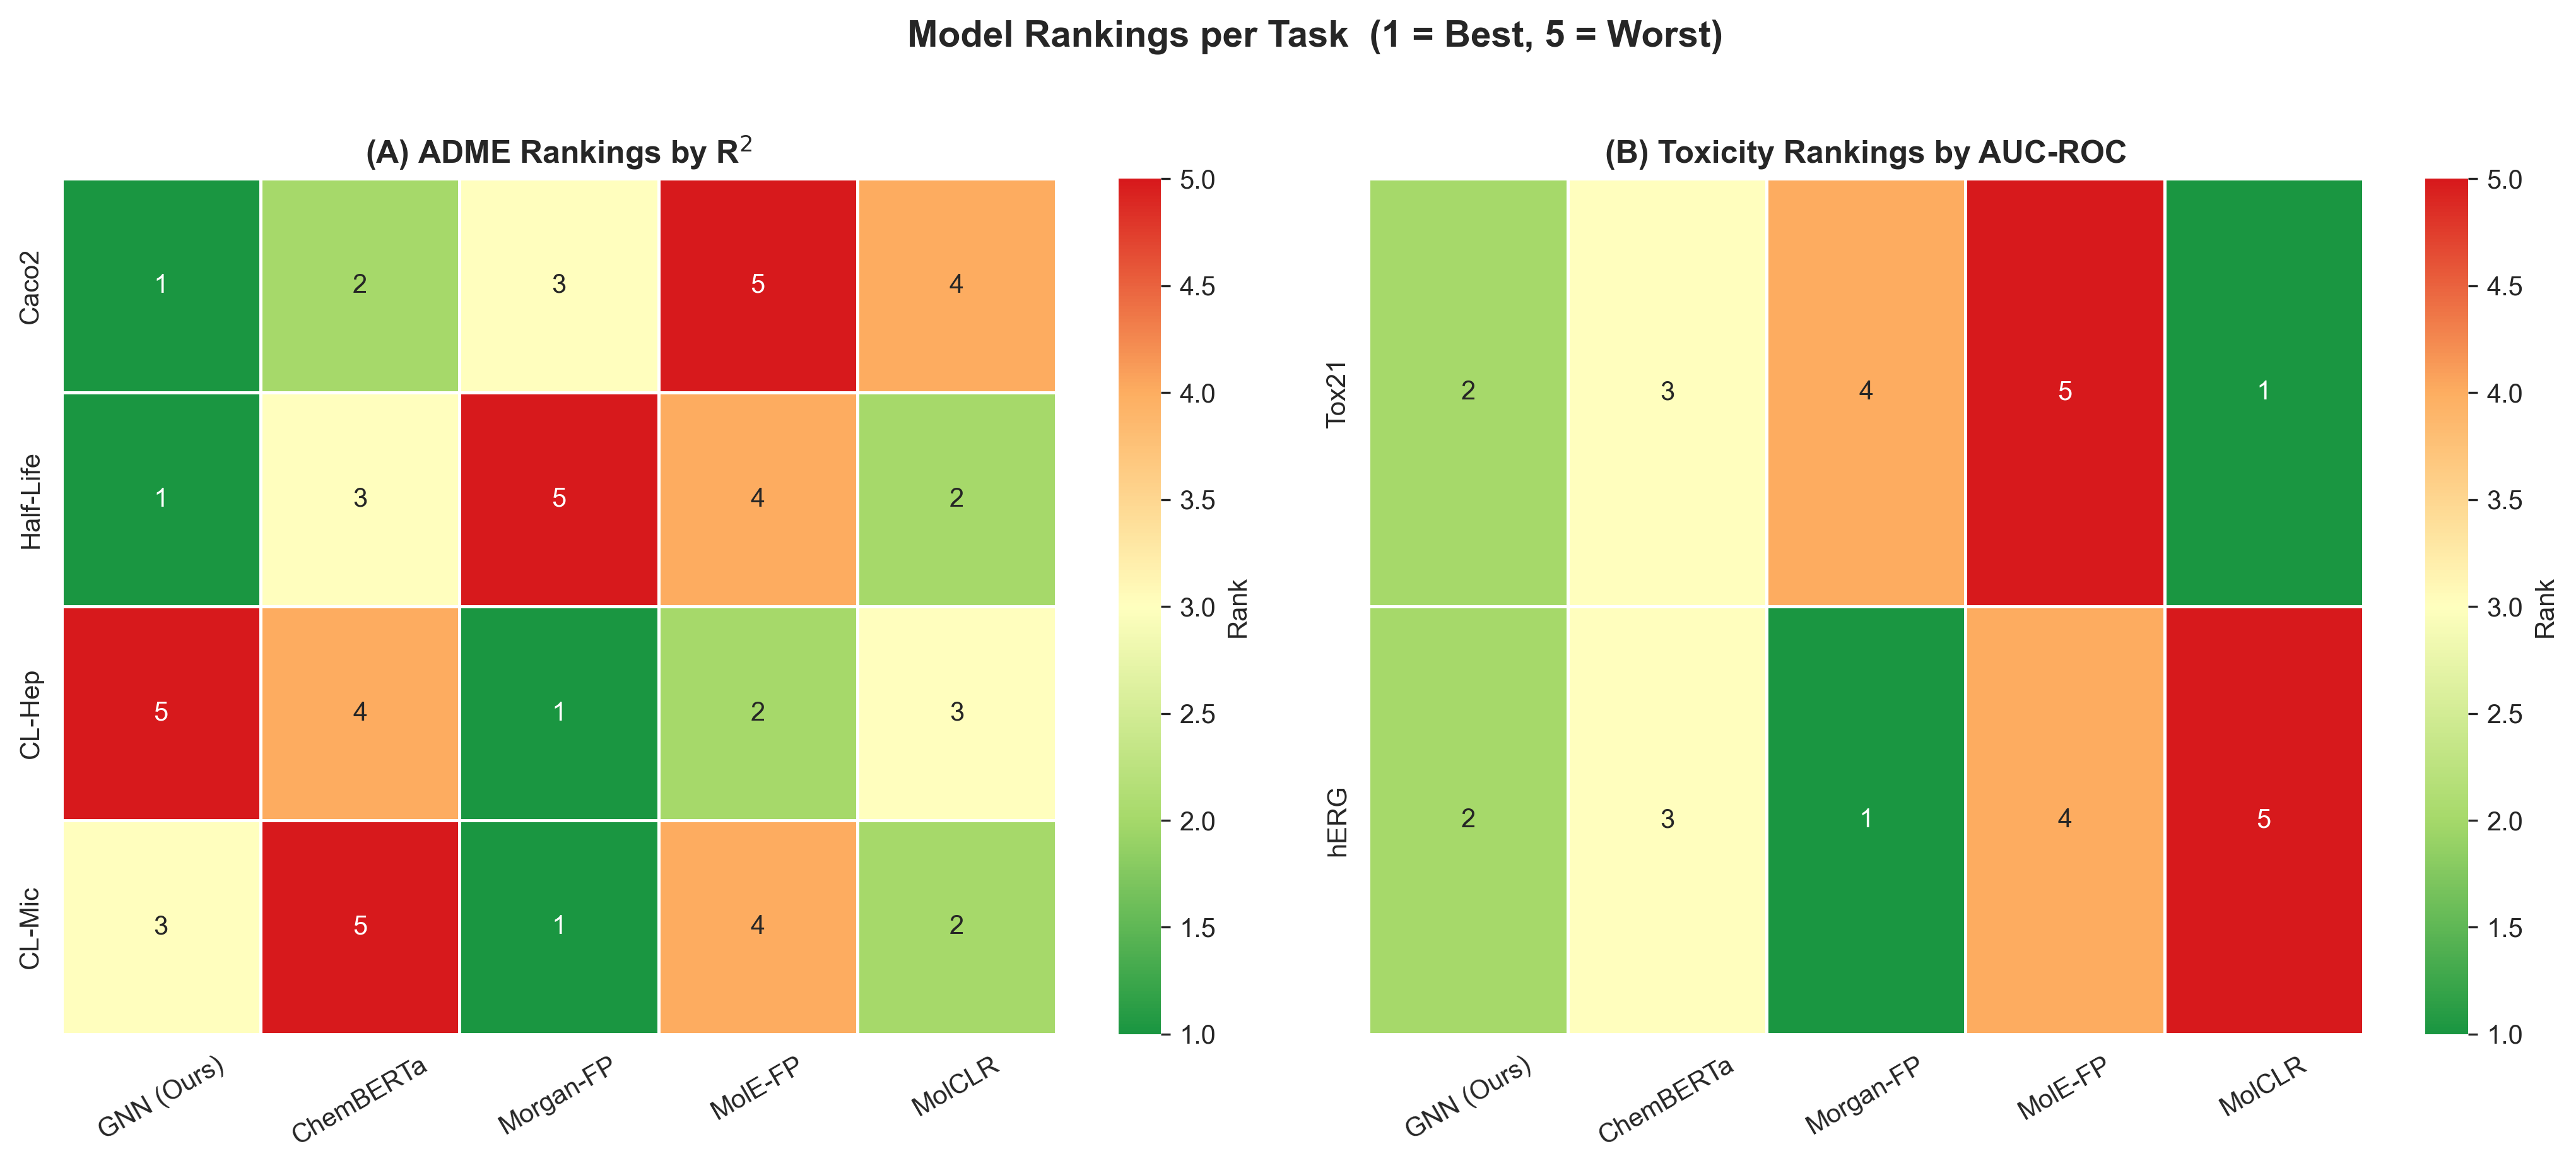
\includegraphics[width=\columnwidth,height=0.42\textheight,keepaspectratio]{foundation_ranking.png}
    \caption{Task-dependent performance of different model families across ADMET endpoints. Green indicates better performance within each task.}
    \label{fig:foundation_ranking}
\end{figure}

\begin{table*}[!t]
\centering
\caption{Fair model-family comparison across ADMET endpoints, reported as the \textbf{median over ten seeds} of each family's validation-selected configuration. Every family receives a matched 50-trial, validation-based tuning budget (GNN: random search over the architecture and training-hyperparameter space; pretrained and fingerprint models: search over the MLP prediction head on frozen features), and each selected configuration is evaluated once on an identical scaffold-split test set; no test information is used for any selection. R$^2$ (regression) and AUC-ROC (classification); higher is better. Bold marks the highest median per endpoint, but the leading families are typically separated by less than the across-seed range, so these should be read as evidence that no family dominates rather than as significant wins. Per-seed ranges are reported in Table~\ref{tab:multiseed}. R$^2$ is scale-invariant across the different target preprocessings; a negative R$^2$ indicates performance worse than the constant predictor equal to the mean of the observed test targets, and on the weakly-learnable clearance and half-life endpoints some validation-selected configurations diverge on a minority of seeds (individual per-seed R$^2$ reaching strongly negative values, reported raw without any capping), which is why medians rather than means are reported.}
\label{tab:model_comparison}
\small
\begin{tabular}{llccccc}
\toprule
\textbf{Task} & \textbf{Metric} & \textbf{GNN} & \textbf{ChemBERTa} & \textbf{Morgan-FP} & \textbf{MolE-FP} & \textbf{MolCLR} \\
\midrule
\multicolumn{7}{l}{\emph{Group 1: Structure-driven tasks}} \\
\midrule
hERG & AUC $\uparrow$ & 0.754 & 0.747 & \textbf{0.767} & 0.735 & 0.657 \\
Caco-2 & R$^2$ $\uparrow$ & \textbf{0.482} & 0.413 & 0.322 & 0.127 & 0.232 \\
\midrule
\multicolumn{7}{l}{\emph{Group 2: Partially structure-driven tasks}} \\
\midrule
Tox21 (NR-AR) & AUC $\uparrow$ & 0.718 & 0.714 & 0.706 & 0.698 & \textbf{0.722} \\
Clearance Mic. & R$^2$ $\uparrow$ & 0.093 & $-$0.010 & \textbf{0.169} & 0.056 & 0.125 \\
\midrule
\multicolumn{7}{l}{\emph{Group 3: Tasks weakly learnable from structure alone}} \\
\midrule
Half-Life & R$^2$ $\uparrow$ & \textbf{$-$0.010} & $-$1.918 & $-$6.341 & $-$3.776 & $-$0.672 \\
Clearance Hep. & R$^2$ $\uparrow$ & $-$0.373 & $-$0.224 & \textbf{$-$0.017} & $-$0.106 & $-$0.113 \\
\bottomrule
\end{tabular}
\end{table*}


We observe substantial variability in predictive performance across tasks, which we organize post-hoc into three groups based on the degree to which molecular structure supports prediction. The grouping is a descriptive summary of the observed test performance on these six endpoints, not a set of universal thresholds: structure-driven endpoints (permeability, direct channel binding) reach the highest scores, endpoints governed by enzyme kinetics, transporter activity, or protein binding sit near or below chance, and the middle group is intermediate. Within every group the leading families are separated by less than the across-seed range, so the central observation is that \emph{no model family dominates}.

\paragraph{Group 1: Structure-driven tasks.}
On hERG and Caco-2 the models reach their highest scores, but no single family is clearly best. On hERG the leading families lie within $0.03$ AUC of one another (Morgan-FP highest at $0.77$, with the GNN and ChemBERTa at $0.75$), a spread smaller than the across-seed range, so we do not read any as a significant winner. On Caco-2 the GNN attains the highest median R$^2$ ($0.48$), but the controlled ablation below shows this advantage comes entirely from the auxiliary physicochemical descriptors: without them the graph model collapses. These endpoints exhibit strong structure--activity relationships---hERG channel blockade is associated with specific pharmacophoric motifs, and intestinal permeability is governed primarily by molecular size, lipophilicity, and hydrogen-bond capacity---which SMILES transformers and fingerprints capture as well as a graph model.

\paragraph{Group 2: Partially structure-driven tasks.}
On Tox21 and Microsomal clearance predictive power is moderate and, again, closely matched. On Tox21 all families lie between AUC $0.70$ and $0.72$ (MolCLR highest at $0.722$, GNN $0.718$); on Microsomal clearance Morgan-FP gives the highest median R$^2$ ($0.17$), ahead of MolCLR ($0.13$) and the GNN ($0.09$). Structure is partially informative here, but no model family dominates.

\paragraph{Group 3: Tasks weakly learnable from structure alone.}
On Half-Life and Hepatocyte clearance, all evaluated models produced weak predictive performance, with near-zero or negative R$^2$ values. The best Half-Life median R$^2$ is only $\approx 0$ ($-0.01$, GNN), while every other family is negative; notably, once the fingerprint baselines are given a full 50-trial tuning budget on these tiny scaffold-split training sets (466 Half-Life molecules), their validation-selected heads overfit and collapse to strongly negative test R$^2$ (Morgan-FP $-$6.3, MolE-FP $-$3.8), a further symptom of how little generalizable signal these endpoints contain. On Hepatocyte clearance the best median is Morgan-FP ($-$0.02); the GNN's validation-selected configuration is unstable on this endpoint and posts a strongly negative median R$^2$ ($-$0.37), with individual seeds reaching strongly negative raw R$^2$ values (Table~\ref{tab:multiseed}). These results suggest that, for the evaluated structure-only representations under scaffold-split evaluation, molecular structure alone provided limited predictive signal for these pharmacokinetic endpoints, which depend on enzyme kinetics, transporter activity, protein binding, and individual patient variability~\cite{obach1999prediction}.

These results suggest that the structure-only representations evaluated here do not, on their own, provide robust predictive performance for endpoints that depend strongly on biological and experimental context under scaffold-split evaluation. Both simple and more complex models showed similarly weak performance on the same endpoints, which is more consistent with a limitation in the information content of the structure-only representation than with the choice of learning algorithm.


\subsection{Model Performance Across Tasks}
\label{sec:model_performance}

We examine performance differences between model families in greater detail using Fig.~\ref{fig:foundation_comparison}, which compares GNN, pretrained, and fingerprint models across all tasks.

\begin{figure*}[!t]
    \centering
    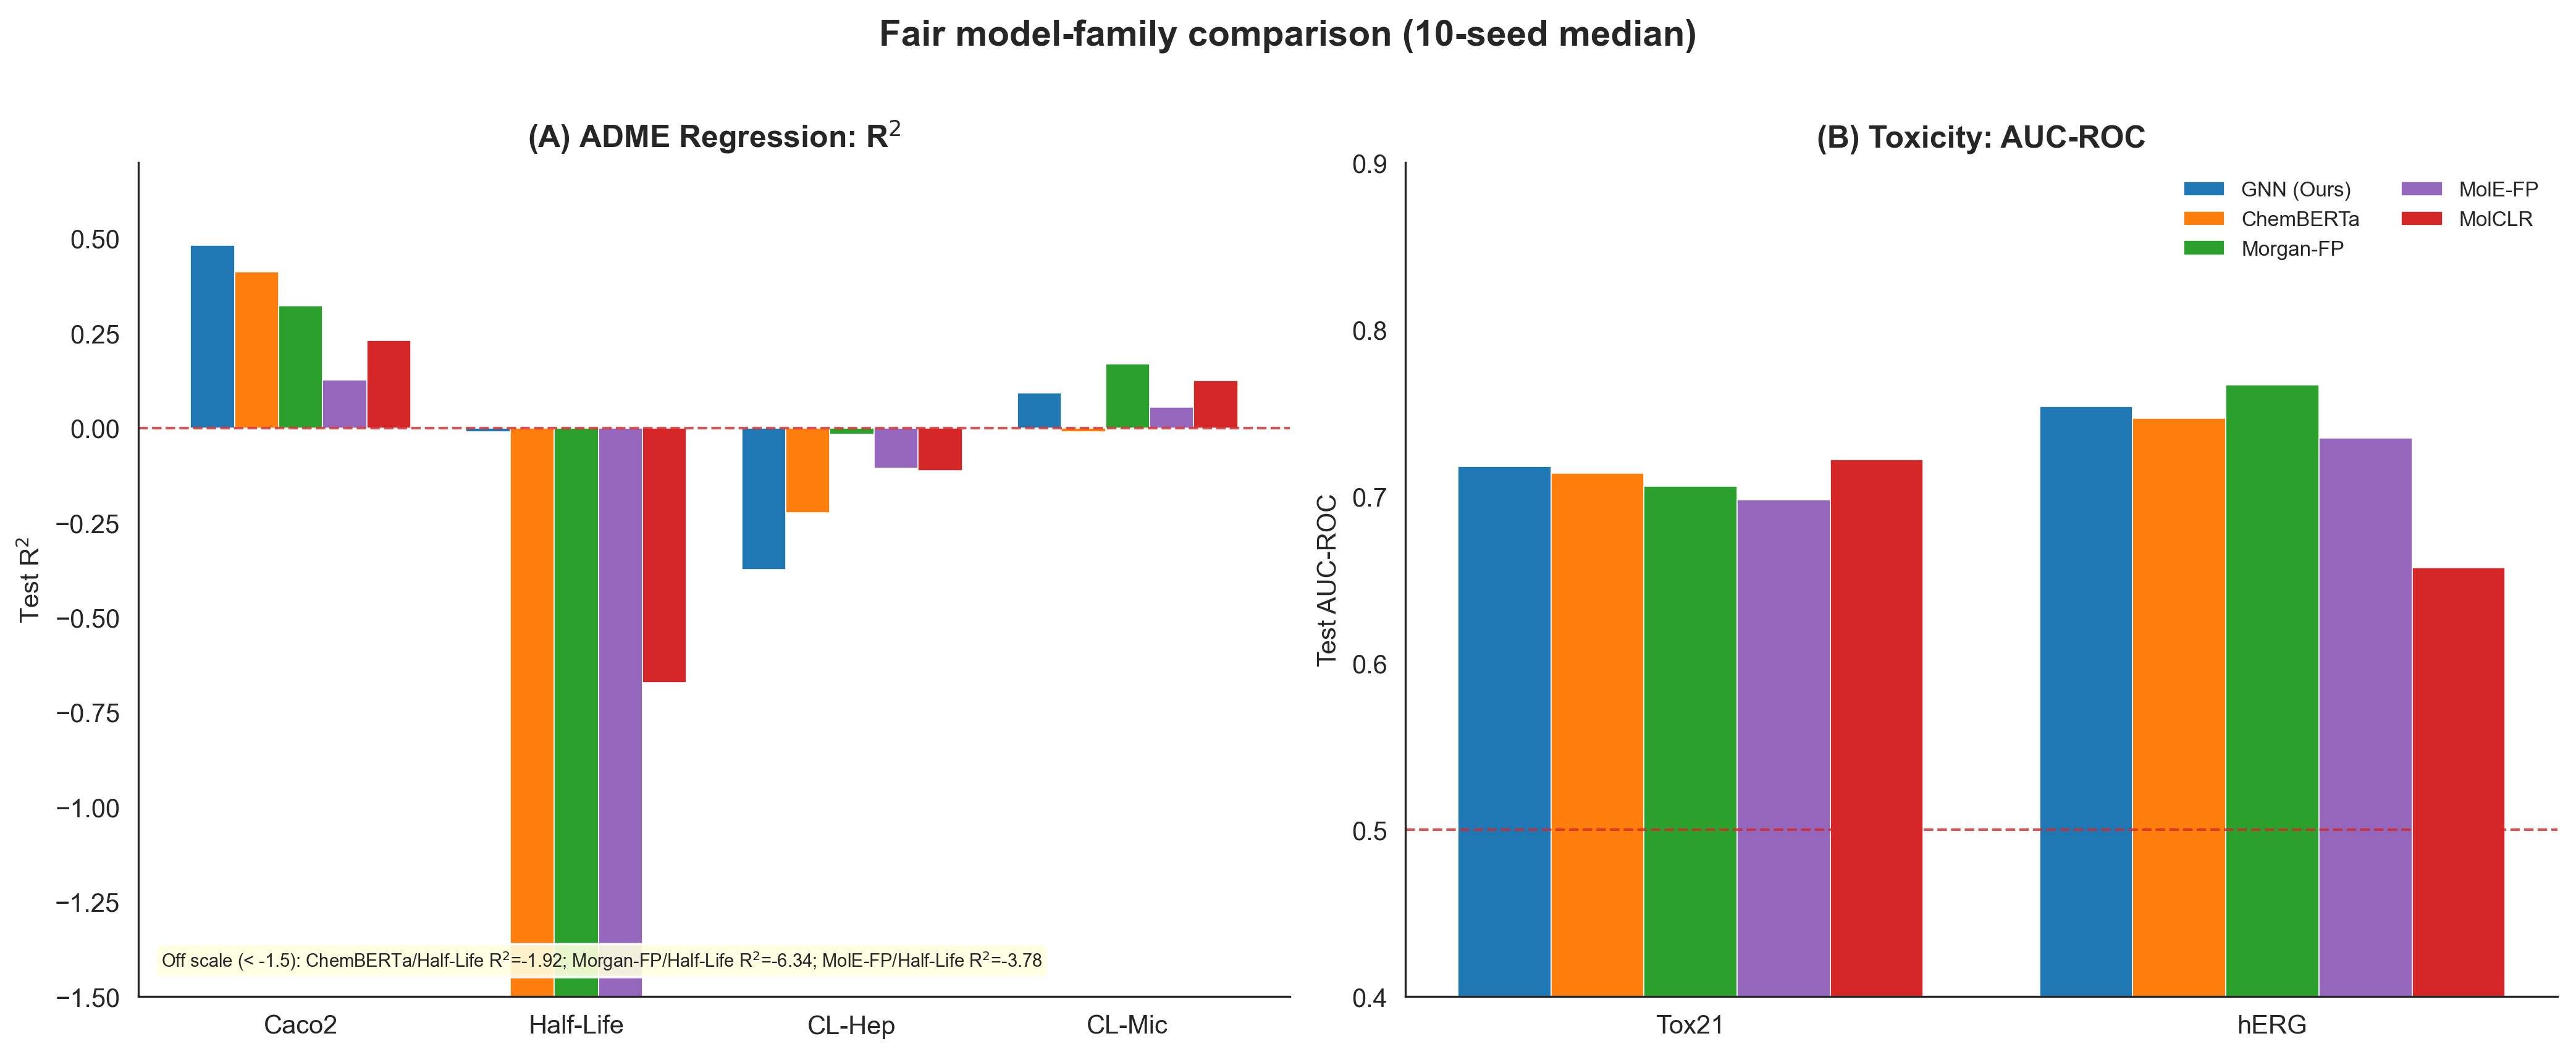
\includegraphics[width=0.95\textwidth,height=0.45\textheight,keepaspectratio]{gnn_vs_foundation_comparison.png}
    \caption{Comparison of GNN (with HPO) against pretrained and fingerprint baselines across all datasets, using the metrics reported in Table~\ref{tab:model_comparison}. (A) ADME regression R$^2$ (higher is better; dashed line at $R^2=0$), (B) toxicity AUC-ROC (dashed line at the 0.5 random baseline).}
    \label{fig:foundation_comparison}
\end{figure*}

\paragraph{Toxicity tasks are closely matched.}
On the two toxicity endpoints no single family is clearly best. On hERG Morgan-FP is highest (AUC = 0.767), with the GNN and ChemBERTa at $\approx 0.75$; on Tox21 MolCLR is highest (0.722), with the GNN at 0.718 and every family between 0.70 and 0.72. Task-specific graph convolution captures substructural motifs, but fingerprints and SMILES transformers capture them comparably here. The GNN additionally receives auxiliary physicochemical descriptors that the frozen baselines do not; the controlled ablation below (Section~\ref{sec:descriptor_ablation}, Table~\ref{tab:descriptor_ablation}) shows these add essentially nothing on the toxicity endpoints (hERG $\Delta \approx +0.00$, Tox21 $\Delta \approx +0.01$), so the GNN's toxicity performance reflects the graph representation rather than the descriptor input.

\paragraph{Permeability: the GNN's one edge is descriptor-driven.}
On Caco-2 the GNN attains the highest median R$^2$ (0.48), ahead of a tuned ChemBERTa (0.41) and Morgan-FP (0.32). As the ablation below shows, this margin comes almost entirely from the auxiliary physicochemical descriptors rather than from the graph representation: without them the graph model collapses (Section~\ref{sec:descriptor_ablation}).

\paragraph{Limited performance on clearance and half-life.}
On Hepatocyte clearance, no evaluated model achieves meaningful predictive power (all R$^2$ near or below zero). The best median is Morgan-FP ($-$0.02), while the GNN's validation-selected configuration is unstable on this endpoint and falls to $-$0.37. The frozen pretrained representations are less extreme than end-to-end GNN training here (a tuned ChemBERTa~\cite{chemberta2} reaches R$^2$ = $-$0.22), which should be interpreted as evidence that frozen representations can serve as regularized baselines in this benchmark, not that pretrained molecular models are generally superior for clearance prediction. On Half-Life and Microsomal clearance, the same pattern of weak or absent predictive signal persists across all model families.

For practitioners, these results indicate a diagnostic approach: if a task-specific GNN achieves negative R$^2$ or near-random AUC on a scaffold-split test set, the endpoint may not be predictable from molecular structure alone, and frozen pretrained encoders can be included as regularized baselines for comparison.

\subsection{Descriptor Ablation}
\label{sec:descriptor_ablation}

Because the GNN alone receives the auxiliary physicochemical descriptors, we run a controlled ablation to separate their contribution from that of the learned graph representation. For each endpoint we take the validation-selected configuration (the GNN column of Table~\ref{tab:model_comparison}) and retrain the GraphConv model twice under an identical training budget (50 epochs, patience 12) and identical seeds, once with the descriptors and once with them removed (the pooled graph embedding is passed directly to the prediction head). These auxiliary descriptors are the GNN's own compact set of RDKit-computed physicochemical features (15 descriptors, or 7 for Caco-2), \emph{not} the separate 200-dimensional RDKit2D block used by the RDKit2D+MLP baseline; the ablation therefore isolates the contribution of this hand-selected descriptor set relative to the learned graph representation. We report the median over ten seeds $[42, 123, 456, 789, 1011, 2022, 3033, 7, 99, 2718]$; because these are re-trained under a fixed shared budget, the with-descriptor column is close to but not identical to the median values in Table~\ref{tab:model_comparison}.

\begin{table}[!t]
\centering
\caption{Descriptor ablation for the GraphConv GNN: test performance with and without the auxiliary physicochemical descriptors, using the validation-selected configuration per endpoint retrained under a matched budget (median over ten seeds). Metric is R$^2$ for regression and AUC-ROC for classification; $\Delta$ is the descriptor contribution (with $-$ without).}
\label{tab:descriptor_ablation}
\small
\setlength{\tabcolsep}{4pt}
\begin{tabular}{llccc}
\toprule
\textbf{Endpoint} & \textbf{Metric} & \textbf{With desc.} & \textbf{Without desc.} & \textbf{$\Delta$} \\
\midrule
Caco-2 & R$^2$ & 0.455 & $-$0.513 & $+0.97$ \\
Half-Life & R$^2$ & 0.037 & 0.013 & $+0.02$ \\
Clearance Hep. & R$^2$ & $-$0.354 & $-$0.040 & $-0.31$ \\
Clearance Mic. & R$^2$ & 0.135 & 0.094 & $+0.04$ \\
Tox21 (NR-AR) & AUC & 0.708 & 0.697 & $+0.01$ \\
hERG & AUC & 0.763 & 0.761 & $+0.00$ \\
\bottomrule
\end{tabular}
\end{table}

The ablation shows that the descriptors are not a uniform bonus but are decisive precisely where the GNN appears strongest. On Caco-2 permeability, removing the descriptors collapses performance from R$^2 = 0.45$ to $-0.51$ ($\Delta = +0.97$): the graph representation alone does not solve this endpoint, and essentially all of the GNN's apparent permeability skill comes from the descriptor vector (which encodes size, lipophilicity, and hydrogen-bonding capacity---exactly the drivers of passive permeability). On the two toxicity endpoints the descriptors contribute essentially nothing ($\Delta \approx +0.00$ AUC on hERG, $+0.01$ on Tox21): the descriptor-free GNN already performs at the level of the fingerprint and pretrained baselines. On the weakly-learnable clearance and half-life endpoints the effect is small or mixed (Half-Life $+0.02$; Hepatocyte clearance $-0.31$, both models near or below zero), consistent with these endpoints being poorly predictable from structure-derived inputs of either kind. These results temper the ``GNNs are best for structure-driven tasks'' reading of Table~\ref{tab:model_comparison}: once tuning and inputs are matched, graph message passing itself confers no consistent advantage, and on Caco-2 the GNN's edge is predominantly descriptor-driven.

\subsection{Backbone Selection}
\label{sec:arch_selection}

A preliminary GNN architecture screen was conducted only to select a practical backbone for the main benchmark, not to establish a definitive ranking of GNN architectures. We evaluated eight common message-passing variants: GCN~\cite{kipf2017gcn}, GAT~\cite{velickovic2018gat}, GraphSAGE~\cite{hamilton2017graphsage}, GIN~\cite{xu2019gin}, TAG~\cite{du2018tagcn}, SGC~\cite{wu2019sgc}, TransformerConv~\cite{shi2021unimp}, and GraphConv~\cite{morris2019wlgnn}. Each architecture was evaluated at its best of five configurations selected on the validation split (varying hidden dimension, number of layers, and learning rate) under the same scaffold-split pipeline used in the main study. Full per-architecture results for both the classification and regression endpoints (all eight backbones) are provided in the supplementary material (Tables~S1 and~S2, Figs.~S1 and~S2).

The screen shows that no single architecture dominates, and that on these datasets the choice of message-passing backbone is largely immaterial. Ranking the eight backbones by \emph{validation} performance---the only selection signal available without touching the test set---the average regression rank spans a narrow band ($3.0$ to $6.0$ across the eight architectures; Table~S2), and the underlying per-dataset validation R$^2$ differences are small (for example, on Caco-2 the eight backbones span validation R$^2 = 0.51$--$0.63$). The two classification endpoints cluster similarly (validation AUC $0.78$--$0.85$ on Tox21 and $0.90$--$0.92$ on hERG; Table~S1). This validation ordering is moreover a poor predictor of test behavior: the best validation-ranked regression backbone (GraphSAGE) reaches only mean test R$^2 = 0.10$, while several validation-competitive backbones (GraphConv, GCN, GIN) post \emph{negative} mean test R$^2$ (down to $-1.57$), and on the weakly-learnable clearance and half-life endpoints every architecture---GraphConv included---is unstable. That instability is a property of the endpoints, not of any backbone, and is itself consistent with this paper's central finding that predictability is endpoint-driven rather than architecture-driven.

Because no backbone is meaningfully better on the validation metric, we did not attempt to identify an ``optimal'' architecture. We instead adopted GraphConv as a single, fixed, representative message-passing backbone for the controlled comparison of model families and hyperparameter-optimization strategies in the main benchmark. GraphConv is mid-ranked on validation (average regression validation rank $4.25$ of $8$, and likewise mid-pack on the classification endpoints; Tables~S1--S2) and is \emph{not} a test-set-maximizing choice---its mean test R$^2$ is in fact among the lowest of the eight backbones. Critically, this selection used validation metrics only and left the test split untouched, so the single test evaluation reported for the main benchmark remains unbiased. We make no claim that GraphConv is architecturally superior: on these small, scaffold-split ADMET datasets the choice of backbone has at most a marginal, within-noise effect on the reported conclusions.


\subsection{Effect of Optimization}
\label{sec:optimization}

Table~\ref{tab:hpo_results} presents the per-optimizer test performance across all tasks, and Table~\ref{tab:best_results} gives the paired statistical comparison of each optimizer against Random Search.

\begin{table*}[!t]
\centering
\caption{HPO-algorithm comparison (clean re-run): test performance of each optimizer's \emph{validation-selected} configuration across datasets (regression R$^2$, classification AUC-ROC). Shown for transparency; optimizers are compared statistically against Random Search in Table~\ref{tab:best_results}, and no optimizer is ever selected using test data. Regression R$^2$ is highly unstable on the weakly-learnable clearance endpoints, so per-optimizer regression values should not be over-interpreted.}
\label{tab:hpo_results}
\scriptsize
\begin{tabular}{lccccccc}
\toprule
\textbf{Dataset} & \textbf{PSO} & \textbf{ABC} & \textbf{GA} & \textbf{SA} & \textbf{HC} & \textbf{Random} & \textbf{TPE} \\
\midrule
\multicolumn{8}{l}{\emph{Regression (R$^2$ $\uparrow$)}} \\
\midrule
Caco2\_Wang & 0.508 & 0.553 & 0.450 & 0.519 & 0.519 & 0.552 & 0.515 \\
Half\_Life\_Obach & 0.119 & 0.211 & 0.193 & $-$0.285 & 0.037 & 0.035 & 0.274 \\
Clearance\_Hep. & $-$0.269 & $-$0.762 & $-$0.219 & $-$1.351 & $-$0.989 & $-$0.114 & $-$0.283 \\
Clearance\_Mic. & 0.235 & $-$0.387 & 0.058 & $-$0.529 & 0.130 & $-$3.288 & $-$0.365 \\
\midrule
\multicolumn{8}{l}{\emph{Classification (AUC-ROC $\uparrow$)}} \\
\midrule
Tox21 (NR-AR) & 0.739 & 0.757 & 0.730 & 0.739 & 0.758 & 0.743 & 0.726 \\
hERG & 0.738 & 0.810 & 0.830 & 0.771 & 0.777 & 0.810 & 0.787 \\
\bottomrule
\end{tabular}
\end{table*}

\begin{table*}[!t]
\centering
\caption{HPO optimizers vs.\ Random Search (clean, leak-free re-run), each optimizer's \emph{validation-selected} configuration evaluated once on test across the $n=6$ datasets. Because the per-endpoint test metrics live on incomparable scales (R$^2$, occasionally pathologically negative, and AUC), we report direction-based and scale-controlled measures rather than a raw mean R$^2$/AUC difference. \textbf{W/T/L}: wins/ties/losses vs.\ Random Search. \textbf{Sign $p$}: exact two-sided binomial test on wins-vs-losses (ties dropped). \textbf{Norm.\ effect}: per-endpoint (optimizer$-$random) difference divided by the spread of all seven optimizers on that endpoint, averaged over the six endpoints (a scale-free, direction-normalized paired effect). \textbf{Sensitivity} columns recompute the mean paired difference with R$^2$ clipped to $[-1,1]$ and floored at $0$ (AUC untouched). All 95\% CIs are $10{,}000$-resample percentile bootstraps over the six paired differences. \emph{No optimizer is significant under the sign test, and every scale-free / clipped interval spans zero}; only the aggressively compressed floor-$0$ variant shows two marginal effects (ABC slightly $+$, SA slightly $-$), neither indicating a consistent winner.}
\label{tab:best_results}
\small
\setlength{\tabcolsep}{4pt}
\begin{tabular}{lccccc}
\toprule
\textbf{Optimizer} & \textbf{W/T/L} & \textbf{Sign $p$} & \textbf{Norm.\ effect [95\% CI]} & \textbf{Clip $[-1,1]$ mean [95\% CI]} & \textbf{Floor-0 mean [95\% CI]} \\
\midrule
PSO & 2/0/4 & 0.69 & $-0.16$ [$-1.35$, $+1.25$] & $+0.174$ [$-0.084$, $+0.612$] & $+0.033$ [$-0.036$, $+0.124$] \\
ABC & 5/0/1 & 0.22 & $+0.52$ [$-0.45$, $+1.38$] & $+0.026$ [$-0.292$, $+0.311$] & $+0.032$ [$+0.000$, $+0.091$] \\
GA  & 3/0/3 & 1.00 & $+0.01$ [$-1.41$, $+1.40$] & $+0.169$ [$-0.067$, $+0.536$] & $+0.020$ [$-0.040$, $+0.086$] \\
SA  & 1/0/5 & 0.22 & $-0.77$ [$-1.82$, $+0.55$] & $-0.135$ [$-0.471$, $+0.171$] & $-0.018$ [$-0.031$, $-0.006$] \\
HC  & 3/0/3 & 1.00 & $+0.02$ [$-1.13$, $+1.37$] & $+0.034$ [$-0.440$, $+0.556$] & $+0.014$ [$-0.021$, $+0.062$] \\
TPE & 2/0/4 & 0.69 & $+0.01$ [$-1.02$, $+1.16$] & $+0.105$ [$-0.075$, $+0.329$] & $+0.027$ [$-0.024$, $+0.114$] \\
\bottomrule
\end{tabular}
\end{table*}

No single optimizer consistently dominates across tasks. Table~\ref{tab:best_results} gives the paired per-endpoint comparison of each optimizer against Random Search, using each endpoint's primary test metric (R$^2$ for regression, AUC-ROC for classification) oriented so that positive values favor the optimizer. None of the metaheuristics shows a consistent net improvement over Random Search: no optimizer is significant under a paired sign test (the most favorable, ABC, wins on five of six endpoints but at $p=0.22$), and every scale-free direction-normalized effect and every scale-clipped mean difference has a bootstrap 95\% confidence interval that spans zero. Only the aggressively compressed floor-$0$ sensitivity variant yields two marginal effects of opposite sign (ABC slightly positive, SA slightly negative), which do not indicate a consistent winner. This indicates that, under our 50-trial budget, optimization strategy has limited impact compared to task characteristics, and that Random Search is a strong baseline rather than one that adaptive search reliably surpasses.

The competitiveness of Random Search on regression tasks is consistent with the ``effective dimensionality'' phenomenon~\cite{bergstra2012random}: when only a subset of hyperparameters (e.g., learning rate, hidden dimension) dominates performance, the probability of Random Search sampling a near-optimal configuration by chance increases. Under such conditions adaptive search has little low-dimensional structure to exploit beyond what random sampling already covers, which is consistent with the absence of a consistent optimizer advantage in Table~\ref{tab:best_results}.



Fig.~\ref{fig:algorithm_performance} compares all algorithms across datasets on test RMSE, R$^2$, and training time; the performance-time panel shows that Random Search and PSO reach competitive accuracy at low computational cost.


The GNN's validation-selected configuration reaches ROC-AUC $>0.7$ on both classification tasks. On hERG it achieves F1 = 0.79 (PR-AUC 0.89, MCC 0.37), with balanced performance across both classes. On Tox21 the same configuration reaches F1 = 0.44 and MCC 0.49 despite high overall accuracy, reflecting the severe class imbalance ($\approx$5\% positive rate on the scaffold-split test set). Per-class confusion matrices are shown in Fig.~\ref{fig:confusion_matrices}.

\begin{figure}[!t]
    \centering
    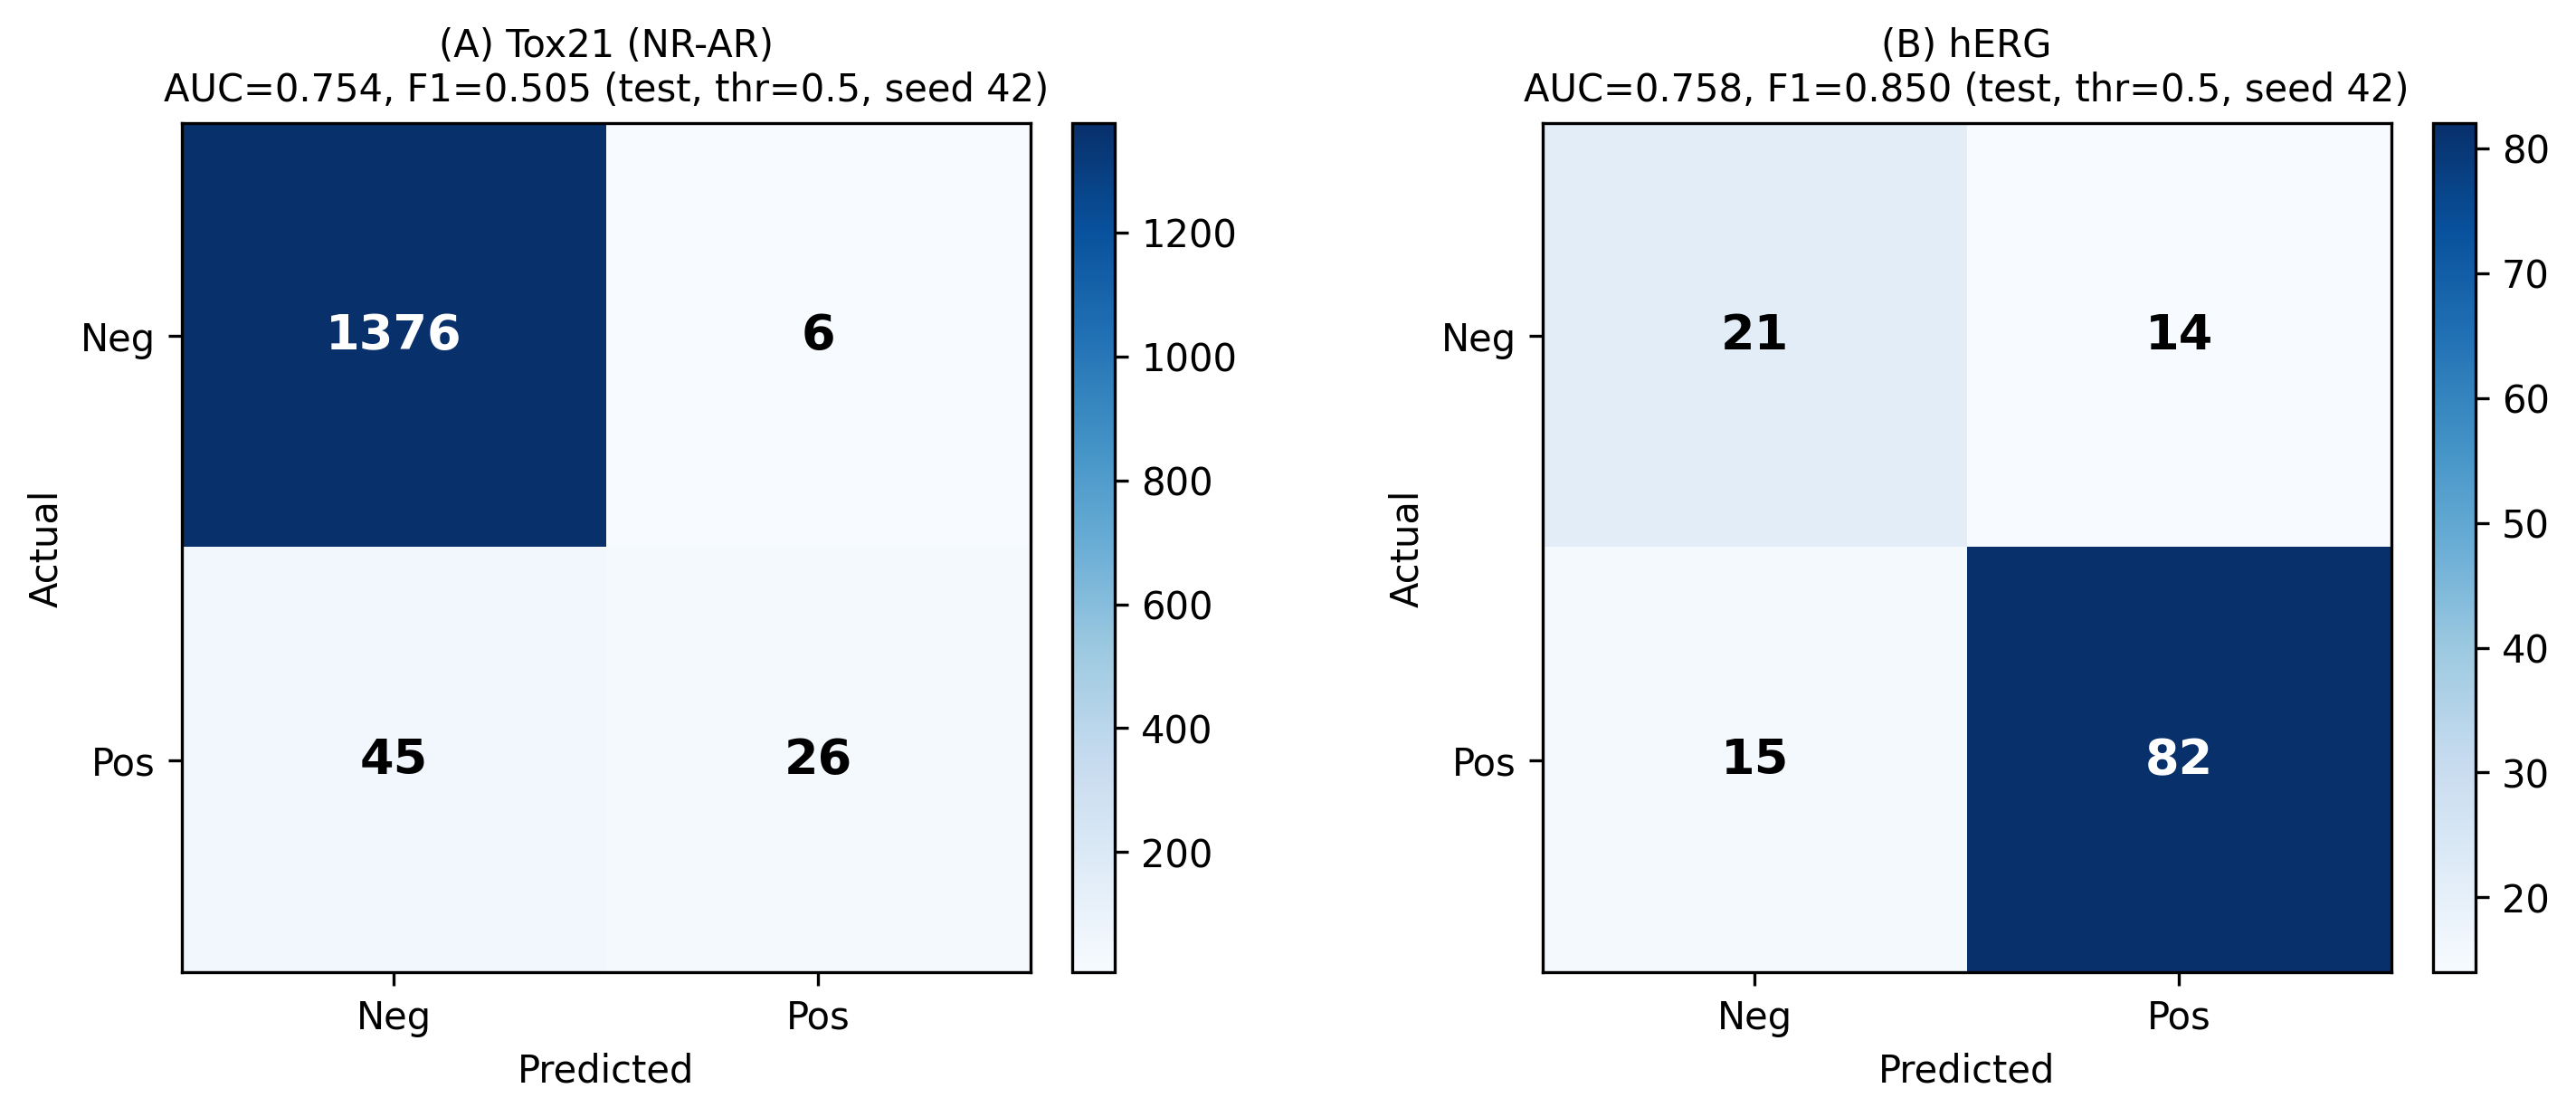
\includegraphics[width=\columnwidth,height=0.28\textheight,keepaspectratio]{confusion_matrices.png}
    \caption{Confusion matrices for the GNN's validation-selected configuration on the two toxicity tasks, on the held-out test set at the standard $0.5$ decision threshold (seed 42). (A) Tox21 shows majority-class bias due to extreme imbalance (F1 = 0.51). (B) hERG shows balanced performance (F1 = 0.85). Across-seed, threshold-tuned aggregates (mean over ten seeds) are reported in the imbalance-metrics table.}
    \label{fig:confusion_matrices}
\end{figure}


\subsection{Imbalance-Aware Metrics and Calibration}
\label{sec:imbalance_metrics}

Because ROC-AUC and accuracy can be misleading under strong class imbalance, we report two further metrics that are sensitive to minority-class behavior: the area under the precision-recall curve (PR-AUC, equivalently average precision) and the Matthews correlation coefficient (MCC)~\cite{chicco2020mcc}. For Tox21 (NR-AR), where positives are only $\approx$5\% of the test set, we regard PR-AUC as a co-primary metric alongside ROC-AUC, since a high ROC-AUC can coexist with weak practical detection of the minority class. PR-AUC is threshold-free and should be compared against the positive-class prevalence, which is the score of a random classifier; the prevalence is $0.049$ for Tox21 (NR-AR) and $0.735$ for hERG on the scaffold-split test set. MCC and F1 are threshold-dependent, so for these two metrics we select the decision threshold that maximizes MCC on the validation split and apply it unchanged to the test split, a standard operating-point selection that never uses test labels. All values are reported as mean $\pm$ standard deviation over the ten seeds $[42, 123, 456, 789, 1011, 2022, 3033, 7, 99, 2718]$ using the GNN's validation-selected configuration per task (the GNN column of Table~\ref{tab:model_comparison}); they complement the ROC-AUC reported in Table~\ref{tab:multiseed}. We deliberately report these bounded, minority-class metrics as mean $\pm$ standard deviation, rather than the median [min--max] used for the ROC-AUC in Table~\ref{tab:multiseed}, because here the across-seed spread is itself the quantity of interest: the standard deviation directly conveys how unstable minority-class performance becomes under class imbalance. The ROC-AUC of Table~\ref{tab:multiseed}, by contrast, is summarized by the median precisely to prevent a single divergent seed from dominating a central-tendency estimate.

\begin{table}[!t]
\centering
\caption{Imbalance-aware toxicity metrics (mean $\pm$ std over $n$=10 seeds), evaluated with the GraphConv backbone. PR-AUC is threshold-free; F1 and MCC use a decision threshold selected on the validation split to maximize MCC. For reference, the PR-AUC of a random classifier equals the positive prevalence (0.049 for Tox21, 0.735 for hERG).}
\label{tab:imbalance_metrics}
\small
\setlength{\tabcolsep}{4pt}
\begin{tabular}{lccc}
\toprule
\textbf{Dataset} & \textbf{PR-AUC} & \textbf{F1} & \textbf{MCC} \\
\midrule
Tox21 (NR-AR) & 0.417 $\pm$ 0.038 & 0.444 $\pm$ 0.063 & 0.493 $\pm$ 0.071 \\
hERG & 0.886 $\pm$ 0.032 & 0.791 $\pm$ 0.090 & 0.373 $\pm$ 0.092 \\
\bottomrule
\end{tabular}
\end{table}

Table~\ref{tab:imbalance_metrics} reports these imbalance-aware metrics. For both endpoints the PR-AUC exceeds the prevalence baseline, indicating that the models recover genuine minority-class signal rather than exploiting the majority class: Tox21 reaches PR-AUC $=0.417$ against a $0.049$ baseline (an $8.5\times$ improvement), and hERG reaches $0.886$ against a $0.735$ baseline. Under validation-based threshold selection the models attain a moderate MCC on both endpoints (Tox21 $0.493$, hERG $0.373$), but with a substantial across-seed spread ($\pm0.071$ and $\pm0.092$), consistent with the difficulty of the $\approx$4.9\% Tox21 positive rate. Minority-class performance is sensitive to the operating point: at the default $0.5$ threshold the Tox21 F1 is markedly lower than after validation-based threshold selection, with some seeds collapsing toward the majority class. This confirms that for severely imbalanced safety endpoints the choice of operating point is as consequential as the choice of model, and that a single threshold-free imbalance-aware metric such as PR-AUC is essential for fair comparison.

Fig.~\ref{fig:toxicity_stability} summarizes the across-seed variability of these metrics. The across-seed spread is modest for both endpoints (for example, PR-AUC $0.417 \pm 0.038$ for Tox21 and $0.886 \pm 0.032$ for hERG), with the threshold-dependent F1 and MCC somewhat more variable on hERG than on Tox21. Fig.~\ref{fig:toxicity_reliability} shows the corresponding reliability diagrams, where the predicted probabilities are pooled over the ten seeds and grouped into ten equal-width bins. Both models are reasonably well calibrated, with Expected Calibration Error of $0.039$ for Tox21 and $0.081$ for hERG, the larger deviations for hERG concentrated at mid-range confidences; this is relevant when predicted probabilities are used directly for risk ranking.

\begin{figure}[!t]
    \centering
    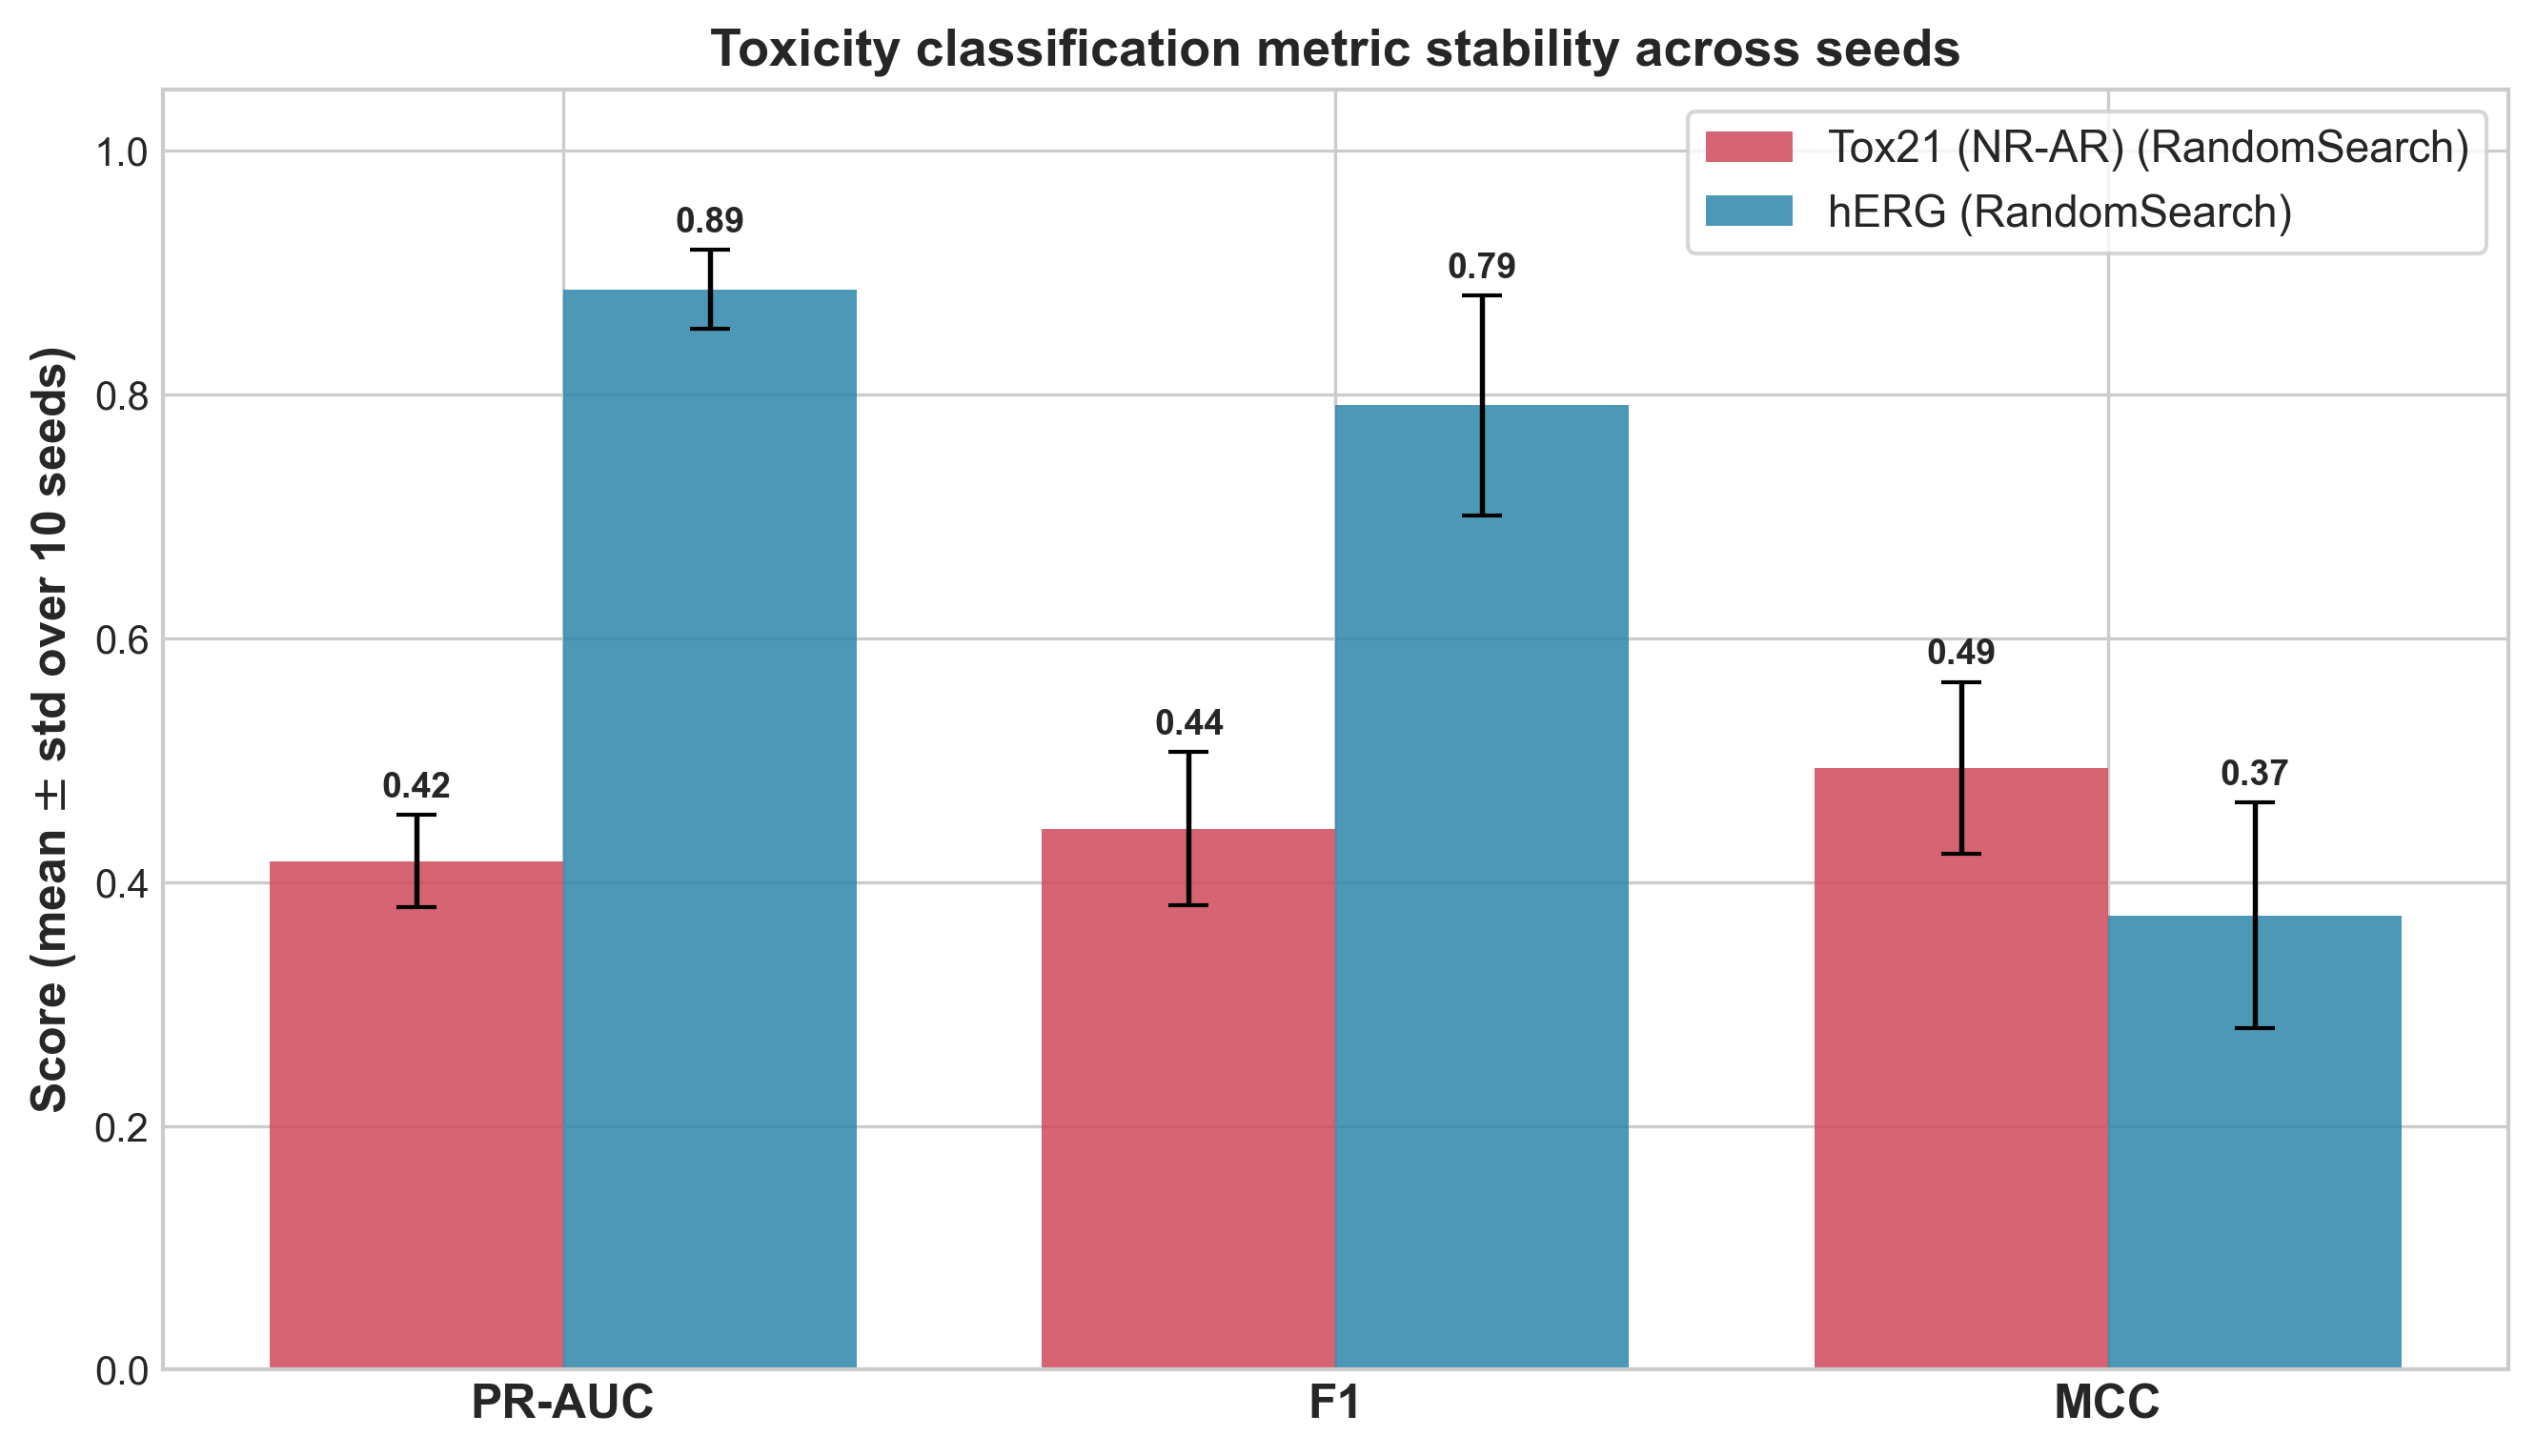
\includegraphics[width=\columnwidth,height=0.30\textheight,keepaspectratio]{toxicity_metric_stability.png}
    \caption{Across-seed stability of the imbalance-aware toxicity metrics (PR-AUC, F1, MCC). Bars show the mean over ten seeds and error bars show $\pm$ one standard deviation. Across-seed variability is modest for both endpoints, with the threshold-dependent F1 and MCC somewhat more variable on hERG than on Tox21.}
    \label{fig:toxicity_stability}
\end{figure}

\begin{figure}[!t]
    \centering
    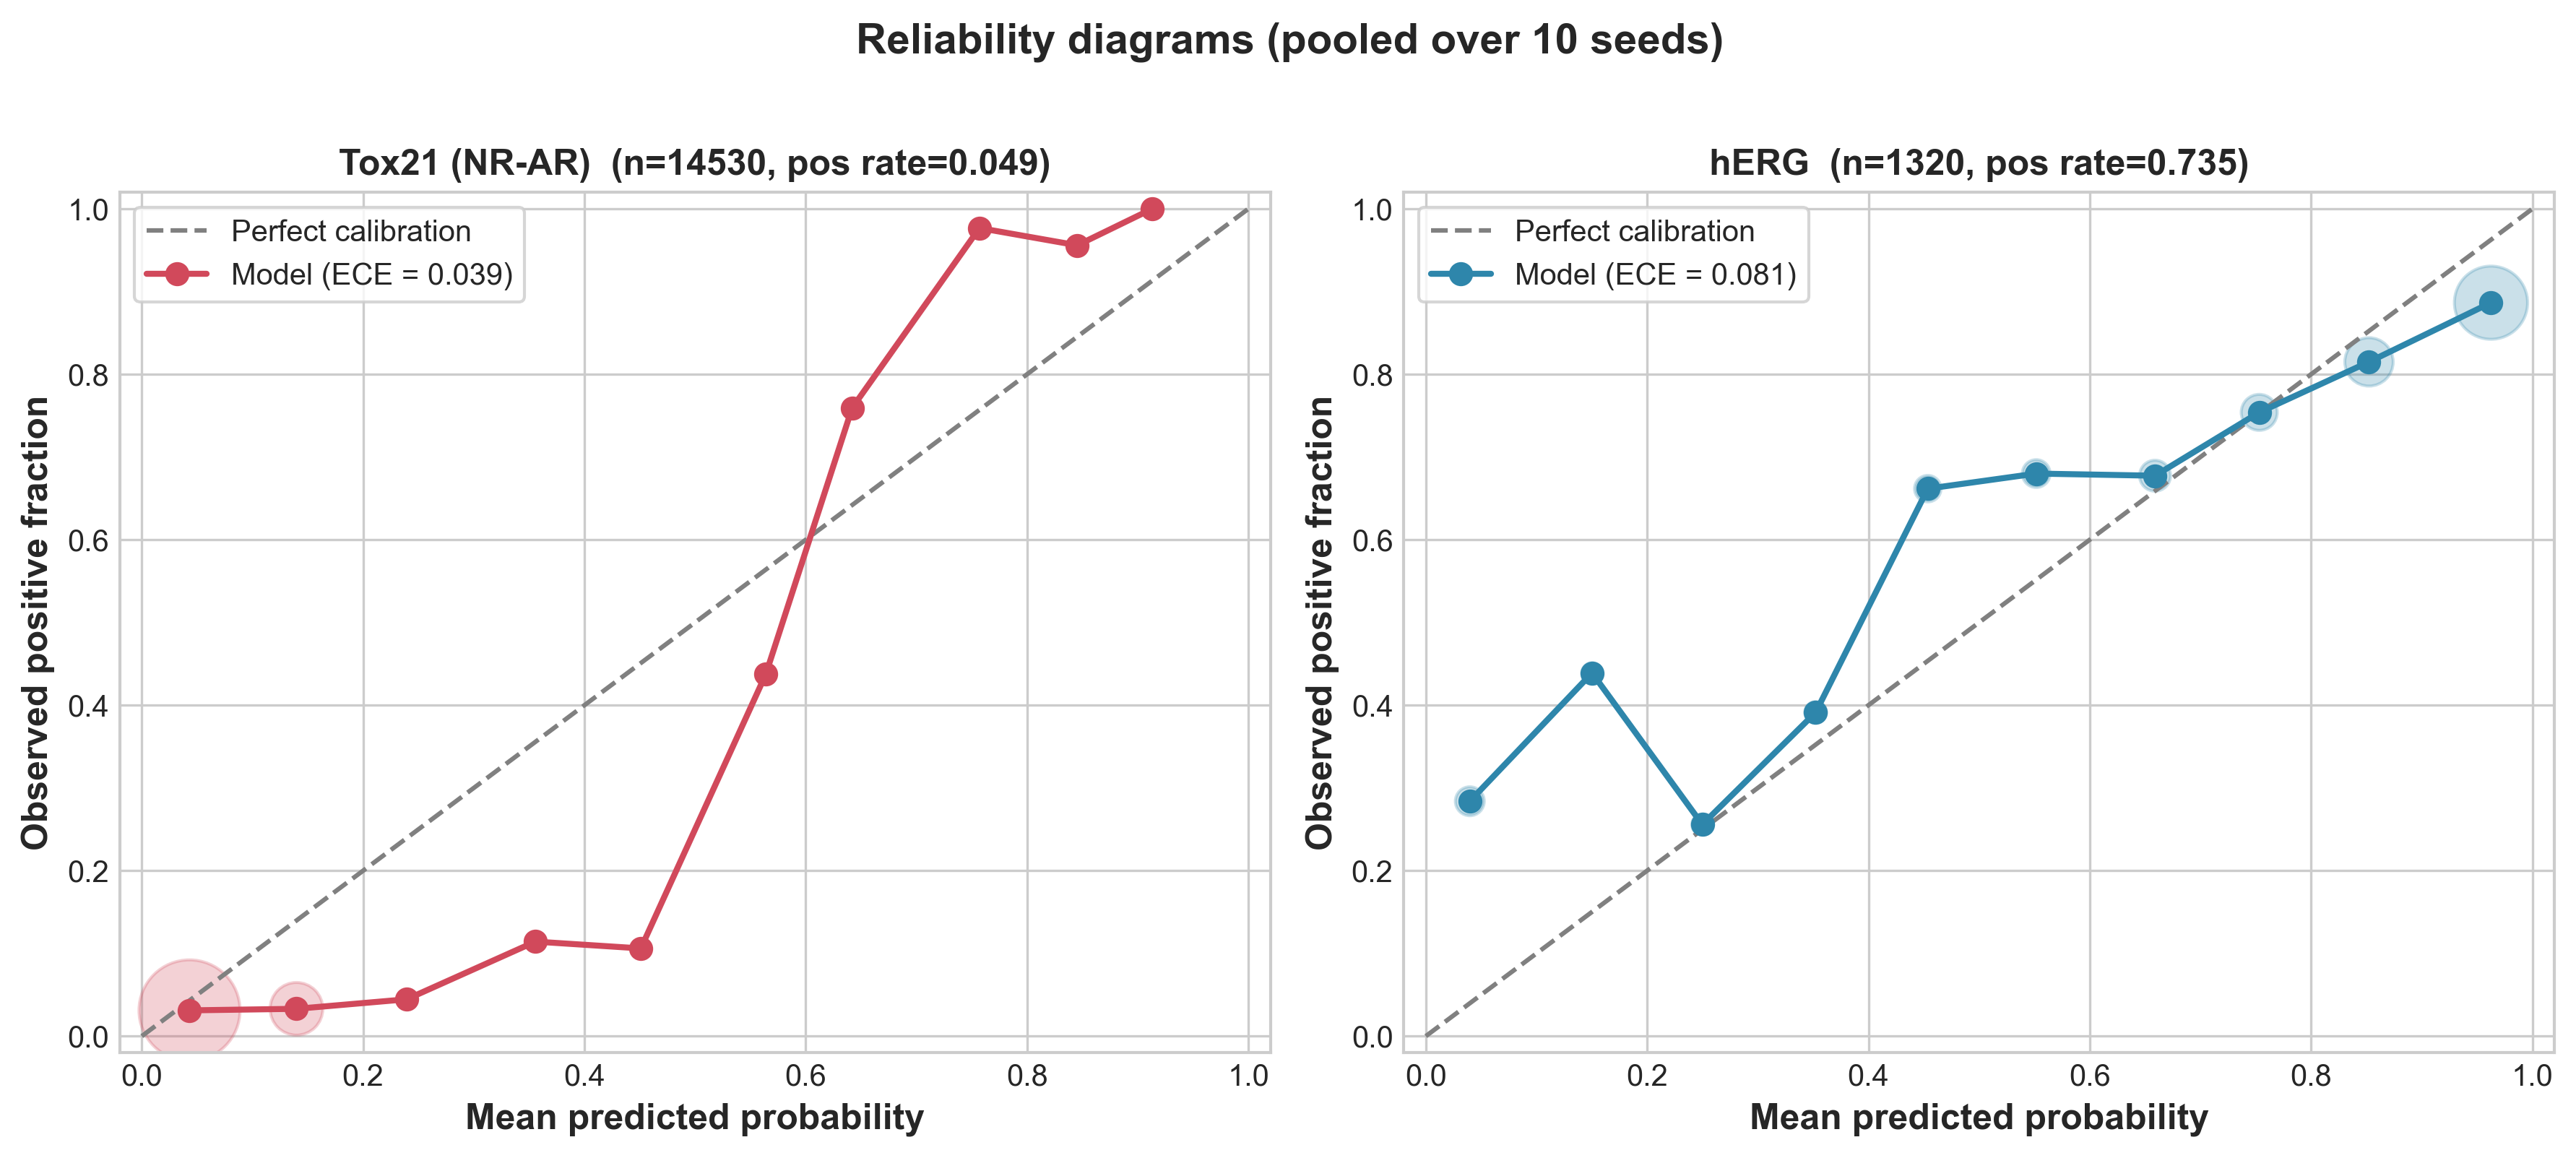
\includegraphics[width=\columnwidth,height=0.30\textheight,keepaspectratio]{toxicity_reliability.png}
    \caption{Reliability diagrams for the toxicity classifiers, with predicted probabilities pooled over ten seeds and binned into ten equal-width intervals. Bubble size is proportional to the number of test molecules in each bin. Both models track the diagonal reasonably closely (ECE $=0.039$ for Tox21, $0.081$ for hERG), indicating reasonably calibrated probabilities.}
    \label{fig:toxicity_reliability}
\end{figure}


\subsection{Effect of Evaluation Protocol}
\label{sec:eval_protocol}

\paragraph{Model-family differences are small under scaffold-split evaluation.}
Table~\ref{tab:multiseed} presents the across-seed variability of the GNN column of Table~\ref{tab:model_comparison} (the validation-selected configuration), evaluated with the GraphConv backbone and reported as the median [min--max] over the ten seeds. Regression is shown as RMSE here to complement the scale-invariant R$^2$ of Table~\ref{tab:model_comparison}. Across-seed stability varies by endpoint and does not simply track structure-drivenness: Caco-2, Microsomal clearance, and hERG (AUC range $0.70$--$0.81$) vary within a relatively narrow band, whereas the configuration diverges on a minority of seeds for Hepatocyte clearance (individual seeds reaching strongly negative R$^2$ and, correspondingly, a very large RMSE). We report the median rather than the mean because the median is robust to these occasional divergent runs; the wide ranges reinforce our central finding that the weakly-learnable pharmacokinetic endpoints do not support robust structure-only prediction. Because the same validation-selected configuration underlies both tables, the multi-seed medians agree with the Table~\ref{tab:model_comparison} values by construction (e.g., hERG AUC median $0.754$, Tox21 $0.718$).

\begin{table}[!t]
\centering
\caption{Across-seed variability of the GNN's validation-selected configuration (the GNN column of Table~\ref{tab:model_comparison}), evaluated with the GraphConv backbone as the median [min--max] over ten seeds $[42, 123, 456, 789, 1011, 2022, 3033, 7, 99, 2718]$. The median is used because the configuration diverges on a minority of seeds for Hepatocyte clearance (individual seeds reaching strongly negative R$^2$); the ranges quantify this instability. Regression is shown as RMSE here to complement the scale-invariant R$^2$ of Table~\ref{tab:model_comparison}.}
\label{tab:multiseed}
\small
\setlength{\tabcolsep}{4pt}
\begin{tabular}{lccc}
\toprule
\textbf{Dataset} & \textbf{Task} & \textbf{Metric} & \textbf{Median [min--max], $n$=10} \\
\midrule
Caco2 & Regr. & RMSE & 0.0027 [0.0025--0.0035] \\
Half\_Life & Regr. & RMSE & 21.80 [18.40--22.86] \\
Clear.\_Hep. & Regr. & RMSE & 56.22 [46.53--977.95] \\
Clear.\_Mic. & Regr. & RMSE & 41.03 [38.48--55.37] \\
Tox21 & Class. & AUC & 0.718 [0.695--0.749] \\
hERG & Class. & AUC & 0.754 [0.704--0.809] \\
\bottomrule
\end{tabular}
\end{table}

\paragraph{Evaluation protocol influences model rankings.}
Scaffold-based splitting creates a structural covariate shift where the model must generalize not merely to unseen molecules, but to unseen chemical families. Under such conditions, validation performance becomes a noisier proxy for true generalization, because a configuration that happens to fit the specific scaffolds in the validation set may not transfer to the test scaffolds. This has important consequences for model selection: on Tox21, the pretrained encoders reach high validation AUC that does not carry over to the scaffold-split test set---ChemBERTa drops from validation AUC $\approx 0.92$ to a test median of $0.714$, and MolCLR from $\approx 0.90$ to $0.722$ (Table~\ref{tab:model_comparison}). These results demonstrate that evaluation protocol substantially influences model rankings and perceived performance.

\paragraph{Partial fine-tuning does not change the picture.}
Because our main comparison uses ChemBERTa as a frozen feature extractor, we tested whether partial fine-tuning closes any gap, extending the check to all six endpoints on the same canonical split as every other model. We fine-tuned ChemBERTa by unfreezing its last two transformer layers (with a class-weighted loss, using train labels only, for the imbalanced Tox21 task). Fine-tuning yields test performance comparable to the frozen-feature protocol---within a few points on the classification endpoints (hERG AUC $0.770$ vs.\ $0.747$ frozen; Tox21 $0.735$ vs.\ $0.714$), positive only on Caco-2 (R$^2 = 0.39$), and near-zero or negative on the harder regression endpoints (Half-Life $-0.08$, Hepatocyte clearance $-0.25$, Microsomal clearance $0.01$). Fine-tuning neither rescues the difficult pharmacokinetic tasks nor overturns the frozen-feature ranking, so the frozen protocol used for the pretrained models does not understate their performance here.

The noise introduced by scaffold splitting also explains why, within the evaluated datasets and 50-trial budget, we did not observe consistent evidence that the evaluated HPO strategies outperform Random Search (Table~\ref{tab:best_results}): no optimizer is significant under a paired sign test, and every scale-free and scale-clipped paired confidence interval spans zero. Adaptive methods use validation performance to guide search decisions; when that signal is noisy, they risk optimizing for the specific validation fold rather than discovering genuinely superior hyperparameters. Random Search, by contrast, does not condition on previous evaluations, making it less susceptible to sequential overfitting of a noisy validation surface.

\begin{figure*}[!t]
    \centering
    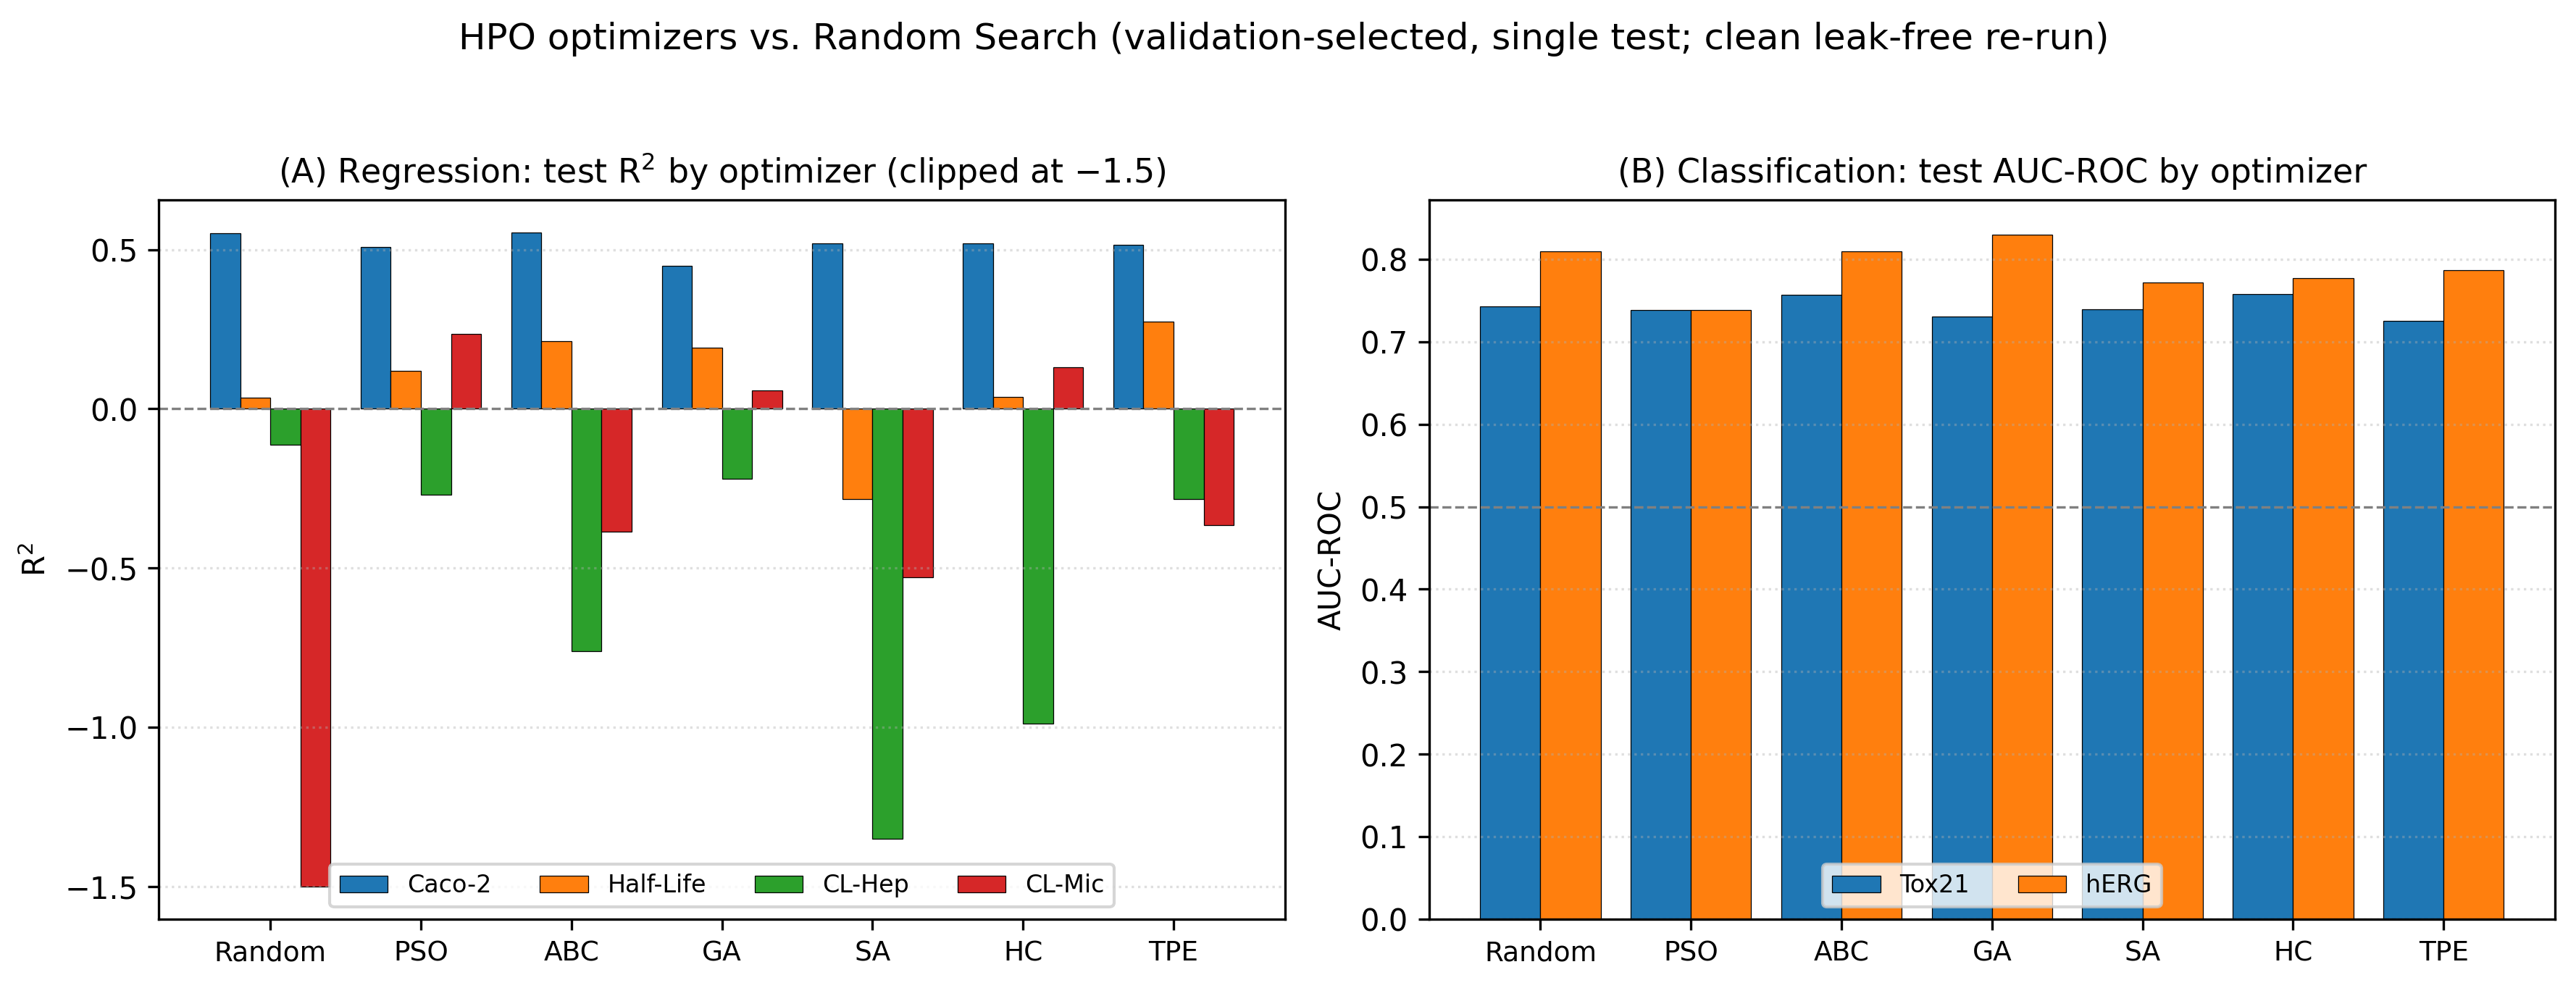
\includegraphics[width=0.95\textwidth,height=0.45\textheight,keepaspectratio]{01_algorithm_performance.png}
    \caption{HPO optimizer comparison (clean, leak-free re-run): each optimizer's \emph{validation-selected} configuration evaluated once on test. (A) Regression test R$^2$ per optimizer across the four ADME endpoints (clipped at $-1.5$ for readability; dashed line at $R^2=0$); (B) classification test AUC-ROC across the two toxicity endpoints (dashed line at the $0.5$ random baseline). No optimizer is consistently ahead of Random Search; see Table~\ref{tab:best_results} for the paired statistics.}
    \label{fig:algorithm_performance}
\end{figure*}

\section{Discussion}
\label{sec:discussion}

Predictive performance varied widely across the six endpoints, from R$^2$ = 0.48 on Caco-2 permeability to a strongly negative median R$^2$ ($-$0.37) on hepatocyte clearance, confirming that ADMET prediction is strongly endpoint-dependent.
Across the evaluated datasets, model rankings were not consistent: architectures that performed well on permeability or toxicity did not necessarily transfer to clearance or half-life prediction.
This indicates that ADMET modeling should not be treated as a single homogeneous prediction problem.
Instead, each endpoint reflects a different combination of physicochemical, biological, and experimental factors, which affects how much predictive signal can be extracted from molecular structure alone.

For endpoints such as Caco-2 permeability and hERG cardiotoxicity, graph-based models achieved competitive performance, suggesting that molecular topology and local chemical environments contain useful predictive information.
This is expected because permeability and ion-channel inhibition are influenced by structural properties such as molecular size, lipophilicity, charge distribution, hydrogen-bonding capacity, and specific functional groups.
In these cases, GNNs can benefit from atom-level message passing over molecular connectivity (our GNN uses atom features and bonds as edges, without explicit bond features), allowing them to capture substructural patterns that are directly relevant to the endpoint; here, however, SMILES transformers and simple fingerprints capture them comparably, and on Caco-2 the graph model's apparent edge derives from auxiliary physicochemical descriptors rather than message passing itself.

In contrast, Half-Life and Hepatocyte clearance showed weak predictive performance across model families, with near-zero or negative \(R^2\) values.
This suggests that these tasks depend on biological and experimental factors not encoded in molecular structure alone, including enzyme-mediated metabolism, transporter interactions, tissue distribution, and plasma protein binding effects~\cite{li2019dmpk,lai2022dmpk,bohnert2013proteinbinding}.
The poor performance on these endpoints is therefore better explained by limitations of structure-only molecular representations than by architecture alone.
In our experiments, increasing model complexity did not compensate for the apparent lack of biological context in the structure-only input representation, consistent with the information required to explain these targets not being captured by molecular structure alone.

The classification results further demonstrate the importance of endpoint-specific evaluation.
Although toxicity and cardiotoxicity tasks are both classification problems, they differ substantially in class balance and biological mechanism.
For example, the Tox21 NR-AR task is highly imbalanced, which can bias standard training objectives toward the majority class~\cite{he2009imbalanced}.
This makes ROC-AUC more appropriate than accuracy for comparing classifiers, but it also means that high AUC values should be interpreted carefully when the positive class is rare.
Future work should therefore evaluate additional metrics such as precision-recall AUC, sensitivity, specificity, and calibration error, particularly for safety-related endpoints where false negatives can be costly.

The scaffold-split protocol also plays an important role in interpreting the results.
Compared with random splitting, scaffold splitting provides a stricter evaluation setting because compounds with the same core scaffold are assigned to the same partition.
This reduces the risk that models exploit close structural analogues in the training set and gives a more realistic estimate of performance on novel chemical series.
The observed performance drops under scaffold-split evaluation therefore highlight the difficulty of generalizing beyond familiar chemotypes, which is a central challenge in practical drug discovery.

The comparison between GNNs, fingerprints, descriptors, and pretrained molecular representation models suggests that no single representation is uniformly optimal.
The frozen pretrained encoders evaluated here can provide useful molecular embeddings, but their performance depends on the alignment between the pretraining objective, the molecular representation, and the downstream endpoint.
Similarly, classical fingerprint-based models remain competitive for some endpoints, especially when the dataset is small or when the target is strongly associated with known physicochemical properties.
These results support endpoint-specific model selection rather than the use of a single architecture across all ADMET tasks.

The hyperparameter optimization results also suggest that optimization should be interpreted cautiously.
None of the evaluated metaheuristics consistently improved on Random Search: no optimizer is significant under a paired sign test, and their scale-free and scale-clipped paired 95\% confidence intervals span zero.
Where individual algorithms win on a particular dataset, the advantage is small and does not transfer across datasets or architectures.
For small and noisy ADMET datasets, validation performance may be unstable, and aggressive optimization can overfit to the validation split.
This reinforces the need for repeated runs, consistent evaluation protocols, and transparent reporting of variance across seeds.
In practice, simple optimization strategies may be sufficient for some endpoints, while more expensive search methods should be justified by consistent improvements across independent runs.

These results support endpoint-specific model selection. Structure-based models are most appropriate for endpoints with clear structure-activity relationships, whereas clearance and half-life prediction likely require additional biological or assay-level variables, including enzyme activity, transporter information, protein binding, and experimental conditions.

In biomedical informatics workflows, ADMET predictors should therefore be interpreted as endpoint-specific decision-support tools rather than interchangeable screening modules. Structure-only models may be useful for hERG and Caco-2 screening, but their predictions for hepatocyte clearance and half-life should be treated cautiously unless additional biological context is available.

This study also has several limitations that bound the scope of our conclusions.
First, the benchmark focuses on six TDC ADMET endpoints, which cover important but not exhaustive aspects of drug safety and pharmacokinetics.
Second, the pretrained encoders (ChemBERTa, MolCLR) are evaluated primarily in a frozen feature-extraction setting rather than under full task-specific fine-tuning; across all six endpoints we additionally applied partial fine-tuning to ChemBERTa (unfreezing the last two transformer layers, on the same canonical split) and found it performed comparably to the frozen baseline---neither consistently better nor worse, remaining within a few points on the classification endpoints and near-zero or negative on the hard regression endpoints (Section~\ref{sec:eval_protocol})---so the frozen setting does not understate its performance on these datasets, though a broader study across additional pretrained encoders remains future work. The pretrained encoders are also treated as representative rather than exhaustive examples of pretrained molecular models.
Third, all model families operate on structure-only inputs, so biological and experimental covariates (assay conditions, metabolizing enzymes, transporter and protein-binding measurements) are not included. We also note that the end-to-end GNN receives, in addition to its learned graph representation, a small vector of structure-derived physicochemical descriptors that the frozen pretrained encoders and fingerprint baselines do not; although these descriptors carry no biological or assay information, the model-family comparison is therefore not strictly input-matched. The controlled descriptor ablation in Section~\ref{sec:descriptor_ablation} (Table~\ref{tab:descriptor_ablation}) quantifies this asymmetry: it accounts for essentially all of the GNN's Caco-2 performance and a smaller $+0.08$ AUC on hERG, so part of the GNN's advantage on the structure-driven endpoints reflects this auxiliary input rather than the graph representation alone.
Fourth, scaffold splitting is a more realistic evaluation protocol than random splitting, but it is still a retrospective benchmark and not a full prospective validation on newly synthesized chemical series.
Fifth, the datasets are small (hundreds to a few thousand compounds) and, for the toxicity tasks, class-imbalanced (e.g., a $\approx$4.2\% positive rate on Tox21 NR-AR), which increases variance across splits and can bias training objectives.
Finally, the hyperparameter optimization comparison is limited to a 50-trial budget per algorithm and dataset; a larger budget could alter the relative standing of the metaheuristics against Random Search.
Accordingly, our conclusions apply within the evaluated datasets, model families, scaffold-split protocol, and frozen/pretrained setup, and further validation on additional datasets and prospective experimental settings would strengthen them.

The benchmark can be extended in three directions.
First, additional ADMET endpoints from the TDC benchmark and external pharmaceutical datasets could be included to test whether the observed endpoint-dependent trends generalize more broadly.
Second, multimodal models that combine molecular graphs with assay metadata, protein targets, enzyme information, or transcriptomic features could be evaluated for endpoints where structure-only representations fail.
Third, uncertainty estimation and calibration should be incorporated to assess not only predictive accuracy but also the reliability of model confidence, which is especially important for safety-critical ADMET applications.


\section{Conclusion}
\label{sec:conclusion}

In this work, we investigated the task-dependent performance of molecular graph neural networks and pretrained representations for ADMET prediction under scaffold-split evaluation. Through approximately 2{,}400 training runs and controlled comparisons across five model families and six TDC ADMET benchmarks, our results show that the usefulness of structure-only molecular models depends strongly on the endpoint being predicted. Structure-only models achieved their strongest performance on endpoints with clearer structure--activity relationships, such as hERG cardiotoxicity (best family AUC $\approx 0.77$) and Caco-2 permeability (R$^2$ = 0.48), yet no single model family dominated even there and the GNN's Caco-2 edge is attributable to auxiliary physicochemical descriptors rather than the graph representation. In contrast, the same modeling approaches failed to provide reliable predictions for pharmacokinetic endpoints such as Half-Life and Hepatocyte Clearance, where both GNNs and pretrained encoders yielded near-zero or negative R$^2$ within the evaluated benchmark.

These results support the main conclusion of this study, that ADMET model selection should be endpoint-specific. Molecular structure is informative for some endpoints, but the structure-only representations evaluated here do not, on their own, yield robust predictions for others under scaffold-split evaluation. We identify three levels of task learnability from molecular structure. First, structure-driven tasks, such as hERG and Caco-2, where the leading families are closely matched---Morgan-FP is highest on hERG, and the GNN on Caco-2, though its edge there is descriptor-driven---and achieve the study's most useful predictions. Second, moderately structure-driven tasks, such as Tox21 NR-AR and Microsomal Clearance, where the model families are closely matched: MolCLR is highest on Tox21 and Morgan-FP on Microsomal Clearance, with the GNN close behind on both. Third, weakly structure-driven tasks, such as Half-Life and Hepatocyte Clearance, where all evaluated models perform poorly regardless of architecture, pretraining, or optimization strategy. This demonstrates that increasing model complexity is beneficial only when the endpoint contains sufficient structure-derived signals.

Scaffold-split evaluation is critical for drawing realistic conclusions from ADMET benchmarks. Random splits can produce overly optimistic estimates by allowing structurally similar molecules to appear in both training and test sets. In contrast, scaffold splitting provides a stricter assessment of generalization to unseen chemical scaffolds. Under scaffold-split evaluation, model-family differences are small and model rankings are endpoint-dependent. We further show that, across the six benchmark datasets and under a 50-trial budget, none of the evaluated metaheuristics consistently outperforms Random Search, with a non-significant paired sign test and scale-free confidence intervals that span zero. This reinforces that evaluation protocol strongly influences the apparent benefit of both model architecture and optimization methods.

This study has several limitations. First, all evaluated models operate on structure-only molecular representations and do not incorporate biological, experimental, or pharmacokinetic context. This likely contributes to the weak performance observed on Half-Life and Hepatocyte Clearance. Second, pretrained models were evaluated primarily in a frozen setting; a partial fine-tuning check across all six endpoints performed comparably to the frozen ChemBERTa baseline (neither consistently better nor worse), so the frozen setting does not understate its performance, though a broader study across additional pretrained encoders remains future work. Third, the conclusions are based on six benchmark datasets of limited size, and results may vary under larger or more diverse ADMET datasets.

Future work should move beyond structure-only prediction by incorporating additional sources of information, including protein targets, assay conditions, experimental metadata, dose-dependent effects, and pharmacokinetic context. Such information may be especially important for endpoints where molecular structure alone is weakly predictive. Further work should also investigate uncertainty-aware model selection and evaluation protocols that better reflect prospective drug discovery settings.

Overall, the strongest contribution of this study is showing that ADMET prediction should not be treated as a single uniform modeling problem. Structure-only models can be effective for endpoints such as hERG and Caco-2, but they fail on endpoints such as Half-Life and Hepatocyte Clearance under scaffold-split evaluation. Therefore, reliable ADMET modeling requires endpoint-specific model selection and realistic scaffold-based evaluation. This supports a cautious use of molecular AI models as decision-support tools in early-stage drug discovery rather than as universally reliable predictors across all ADMET endpoints.


\section*{Data and Code Availability}
All datasets used in this study are publicly available through the Therapeutics Data Commons (TDC). The source code, trained model configurations, hyperparameter-optimization logs, and experimental results are available at:
\begin{center}
\url{https://github.com/NitramVonemats/ADMET-Benchmark}
\end{center}

Multi-seed validation used the fixed seeds $[42, 123, 456, 789, 1011, 2022, 3033, 7, 99, 2718]$, and each HPO algorithm was run for 50 trials per dataset. Software dependencies and exact versions are documented in the repository, including Python~$\geq$~3.8, PyTorch~$\geq$~2.0, PyTorch Geometric, RDKit, PyTDC, NiaPy, Optuna, and Transformers.

\section*{Ethical Compliance}
This study uses only publicly available benchmark datasets from the Therapeutics Data Commons and does not involve human subjects, identifiable patient data, animal experiments, or newly collected clinical data. Therefore, institutional review board approval and informed consent were not required.

\bibliographystyle{IEEEtran}
\bibliography{refs}

\end{document}